\documentclass[12pt,a4paper,oneside,english]{report}
\usepackage[square,sort,comma,numbers]{natbib} 
\usepackage[hscale=0.75,vscale=0.85,bindingoffset=0.5cm,includeheadfoot,a4paper, margin=1.5cm]{geometry}
\usepackage{subfigure} 
% \usepackage{cite}
\usepackage{graphicx,type1cm,eso-pic,color}
\usepackage{changepage}
%\usepackage{graphicx}
\usepackage{amsmath, amsthm, amssymb}
\newcommand\norm[1]{\left\lVert#1\right\rVert}
\usepackage[lined,ruled,linesnumbered]{algorithm2e} % vertical lines for if/for/while..., box, chapter-wise numbering
\usepackage[T1]{fontenc}
\usepackage{booktabs}
\usepackage{tabularx}
% \usepackage{tabularx}
\usepackage{longtable}
\usepackage{caption}
\usepackage{multicol}
\usepackage[latin9,utf8]{inputenc}
\usepackage[english]{babel}
\usepackage{amssymb} 
\usepackage{setspace} 
\usepackage{fancyhdr}
\usepackage{lineno}
\usepackage{color}
\usepackage{enumerate}
\usepackage[font=sf, labelfont={sf,bf}]{caption}
\usepackage{draftcopy}
\usepackage[nottoc,notlof]{tocbibind}
\usepackage{fncychap}
\usepackage{fancybox}
\usepackage{threeparttable}
\usepackage{multirow}
\usepackage{graphicx}
\usepackage{mwe}
\usepackage{algorithmic}
%\usepackage[lined,ruled,linenumbered]{algorithm2e}
\usepackage[numbers]{natbib}
%\renewcommand\refname{References}
\newcommand{\comm}


\renewcommand{\baselinestretch}{1.5}
\newtheorem{theorem}{Property}[chapter]




% ---------------- Paragraph Spacing -------
\setlength{\parskip}{1ex}

% ---------------- Format headings and sub-headings -------
\comm{
\makeatletter
\renewcommand\section{\@startsection {section}{1}{\z@}%
                                   {-3.5ex \@plus -1ex \@minus -.2ex}%
                                   {2.3ex \@plus.2ex}%
                                   {\centering\normalfont\LARGE\bfseries}}
                                   
\renewcommand\subsection{\@startsection {subsection}{1}{\z@}%
                                   {-3.5ex \@plus -1ex \@minus -.2ex}%
                                   {2.3ex \@plus.2ex}%
                                   {\centering\normalfont\Large\bfseries}}
                                   
\renewcommand\subsubsection{\@startsection {subsubsection}{1}{\z@}%
                                   {-3.5ex \@plus -1ex \@minus -.2ex}%
                                   {2.3ex \@plus.2ex}%
                                   {\centering\normalfont\large\bfseries}}
\makeatother


% -------------- TOC and TOF Style -------------------------
\makeatletter

\renewcommand{\@pnumwidth}{1.5em}
\renewcommand{\@tocrmarg}{1.55em plus1fil} 
\renewcommand{\@dotsep}{0.9} 
\makeatother

\setcounter{secnumdepth}{2}
\setcounter{tocdepth}{3}
\setcounter{lofdepth}{1}
\setcounter{secnumdepth}{5}
}

% -------------- figure Style -------------------------
%The larger the first two parameters and the smaller the last one, the more a page can be filled with figures and the less has to be text.
\comm{
\renewcommand{\topfraction}{.9}
\renewcommand{\bottomfraction}{.9}
\renewcommand{\textfraction}{.1}

% -------------- Subfigure Style -------------------------
\renewcommand{\thesubfigure}{\thefigure.\arabic{subfigure}} 
\makeatletter 
\renewcommand{\p@subfigure}{} 
\renewcommand{\@thesubfigure}{\thesubfigure:\hskip\subfiglabelskip} 
\makeatother 


%%%  ----- Table style ---- %%%%%%%%%%%%%%%%%%%%%%%%%%%
\renewcommand{\tabcolsep}{0.5cm}
\renewcommand{\arraystretch}{1.5}
}

%%%  ----- Fancy Header ---- %%%%%%%%%%%%%%%%%%%%%%%%%%%

\pagestyle{fancy}
%\renewcommand{\chaptermark}[1]{\markboth{Chapter \thechapter:\ #1}{}}
\renewcommand{\chaptermark}[1]{\markboth{\MakeUppercase{Chapter \thechapter}}{}}
\renewcommand{\sectionmark}[1]{\markright{\MakeUppercase{\thesection\ #1}}}
\renewcommand{\subsectionmark}[1]{\markright{\MakeUppercase{\thesubsection.\ #1}}}
\renewcommand{\subsubsectionmark}[1]{\markright{\MakeUppercase{\thesubsubsection.\ #1}}}

\fancyhf{}
\fancyhead[RO]{\rightmark} % fancy header alignment LO- left order side RO- right order side
%\fancyhead[]{\leftmark}
%\fancyhead[LO]{\leftmark}
\fancyfoot[R]{\thepage} %page number alignment L-leftside , R-rightside, M-middle 
\renewcommand{\headrulewidth}{0pt}
\renewcommand{\footrulewidth}{0pt}
\addtolength{\headheight}{0.9pt}
\fancypagestyle{plain}{
  \fancyhead{}
  \renewcommand{\headrulewidth}{0pt}
}

%%%  ----- In input file ---- %%%%%%%%%%%%%%%%%%%%%%%%%%%

%\input{../Latex/MacroFile1}

%%%  ----- to restrict hyphenation  ---- %%%%%%%%

\hyphenpenalty=5000
\tolerance=1000


%%%  ----- pdf style ---- %%%%%%%%

\ifpdf
    \usepackage[ pdftex, plainpages = false, pdfpagelabels, 
                 pdfpagelayout = useoutlines,
                 bookmarks,
                 bookmarksopen = true,
                 bookmarksnumbered = true,
                 breaklinks = true,
                 linktocpage = true,
                 pagebackref,
                 colorlinks = false,  % was true
                 linkcolor = blue,
                 urlcolor  = blue,
                 citecolor = red,
                 anchorcolor = green,
                 hyperindex = true,
                 hyperfigures
                 ]{hyperref} 
\fi

%%% ----------    begin document --------------



\begin{document}

\pagenumbering{roman}

% \newpage
% %-------------------hard cover page form the thsis
% \thispagestyle{empty}
% \thispagestyle{empty}
% \begin{center}
% 	\vspace*{-2cm}  
% 	{\Large \bf MASTERS THESIS\\}
% 	\vspace*{0.5cm}
% 	{\Large \textbf{Hypergraph-driven Semi-Supervised learning approaches for
% variants of SVMs}\\}
	
% 	\vspace*{1.1cm}
% 	\large by \\\vspace{-.2cm}
% 	Dev Nirwal
	
% 	\vspace*{0.8cm}
% 	{Under the Supervision of}\\\vspace{-.2cm}Dr. Reshma Rastogi
% 	\\
	
% 	\vspace*{0.8cm}
	
% 	Submitted in partial fulfillment of the requirements\\ \vspace{-.2cm} for the award of the degree of\\\vspace{-.2cm}
% 	Master of Science in Computer Science\\
% 	\vspace{0.4cm}
% 	to the
% 	\vspace{0.7cm}
% 	\begin{center}
% 		\includegraphics[scale=0.5]{Figures/SAULOGO.jpg}
% 	\end{center}
% 	\vspace*{0.55cm}
% 	\textbf{   {DEPARTMENT OF COMPUTER SCIENCE \\}\vspace{-.2cm}
% 		\hspace{-0.4cm}{ FACULTY OF MATHEMATICS AND COMPUTER SCIENCE \\}\vspace{-.2cm}
% 		\hspace{-0.4cm}{  SOUTH ASIAN UNIVERSITY, NEW DELHI - 110068, INDIA}\vspace{-.2cm}
% 		{ \\December, 2024}
% 	}
% 	%\vspace*{0.5cm}
% 	\vspace*{0.3cm}   
% 	\vfill
% \end{center}

%------------ front page of main thesis------
\newpage
\thispagestyle{empty}
\begin{center}
	\vspace*{-2cm}  
	{\Large \bf MASTERS THESIS\\}
	\vspace*{0.8cm}
	{\Large \textbf{Hypergraph-driven  Semi-Supervised  learning approaches for variants of SVMs}\\}

	\vspace*{0.6cm}
	\textit{by}

	\vspace{0.4cm}

	{ \large Dev Nirwal } 
	
	\vspace*{0.9cm}
	{ \it Under the Supervision of}\\{\large Dr. Reshma Rastogi}
	\\
	
	\vspace*{0.9cm}
	
	\textit{Submitted in partial fulfillment of the requirements for the award of the degree of}\\
	\textbf{\large  Master of Science in Computer Science}\\
	\vspace{0.6cm}
	\textit{to the}
	\vspace{0.6cm}
	\begin{center}
		\includegraphics[scale=0.55]{Figures/SAULOGO.jpg}
	\end{center}
	\vspace*{0.8cm}
	\large \textbf{     {Department of Computer Science \\}\vspace{-.2cm}
		{ Faculty of Mathematics and Computer 110068, India\\}\vspace{-.2cm}
		{ December, 2024}
	}
	%\vspace*{0.9cm}
	\vspace*{0.3cm}   
	\vfill
\end{center}

%----------copyright page------------
\newpage
\thispagestyle{empty}
 \vspace*{4cm}
\vfill{}
\hspace{-0.8cm} \textbf{\copyright \hspace{0.1mm} South Asian University, 2024\\
	All Rights Reserved.}
\vspace{-2cm}

%---------------Certificate------------will be provided by  yout supervisor
\newpage
\begin{center}
	\huge{\textbf{Certificate}}\\[1.5cm]
\end{center}
%\chapter*{Declaration}
\addcontentsline{toc}{chapter}{Certificate}
This is to certify that the thesis entitled "\textbf{Hypergraph-driven  Semi-Supervised learning approaches for variants of SVMs}" submitted by \textbf{Dev Nirwal} (Enrollment No. SAU/CS(M)/2022/03) the Department of Computer Science, Faculty of Mathematics and Computer Science, South Asian University, New Delhi, 110068, India in partial fulfilment of the requirements for the award of the degree of \textbf{Master of Science in Computer Science}, is a record of the bonafide work carried out by him under my supervision and guidance.\par

The results contained in this thesis have not been submitted in part or full to any other university or institute for the award of any degree diploma.


\vspace{1.9cm}

\begin{flushright} 
	Dr. Reshma Rastogi\\
	(Supervisor)\\
	Department of Computer Science\\
	Faculty of Mathematics and Computer Science\\
	South Asian University, New Delhi, India\\
	December,2024
\end{flushright} 


% --------------Declaration------------------------------------------------
\newpage
\begin{center}
	\huge{\textbf{Declaration}}\\[1.5cm]
\end{center}
%\chapter*{Declaration}
\addcontentsline{toc}{chapter}{Declaration}
I hereby declare that the thesis entitled "\textbf{Hypergraph-driven  Semi-Supervised  learning approaches for variants of SVMs}" being submitted to the Department of Computer Science, Faculty of Mathematics and Computer Science, South Asian University, New Delhi in partial fulfilment of the requirements for the award of the degree of \textbf{Master of Science in Computer Science} contains the original work carried out by me under the supervision of Dr. Reshma Rastogi. The research work reported in this thesis is original and has not been submitted either in part or full to any university or institution for the award of any degree or diploma.

\vspace{1.9cm}

\begin{flushright} 
    
	Dev Nirwal\\
	SAU/CS(M)/2022/03 
\end{flushright} 


% ---------------------------------------------------------------------------------------
\newpage
%\large
\begin{center}
	\huge{\textbf{Acknowledgement}}\\[1.5cm]
\end{center}
%\chapter*{Acknowledgement}
\addcontentsline{toc}{chapter}{Acknowledgement}

%\vspace{-1.7cm}

First and foremost, I would like to thank my supervisor, Dr Reshma Rastogi, for her continuous optimism concerning this work, providing me with excellent guidance and atmosphere for this project. She let me experience the research and deal with the practical issues beyond the textbooks, patiently corrected my mistakes and helped me develop my background in machine learning.

I would also like to thank my colleague-junior-brother like friend Ankush Bisht and my lab-mates Dr Sanjay Kumar, Sambhav Jain and Mamta Bhattarai Lamsal, and Sayanta Chowdhury for always cheering me up and supporting me throughout.

\vspace{0.3cm}

\begin{flushright} 
	Dev Nirwal  \\
	SAU/CS(M)/2022/03 \\
	December, 2024
\end{flushright} 

%-----------------------------------



\newpage
%\large
\begin{center}
	\huge{\textbf{Abstract}}\\[1.5cm]
\end{center}
This dissertation explores and extends existing work by developing two novel semi-supervised frameworks based on applications of hypergraphs in machine learning. Improved Hypergraph Laplacian Support Vector Machine (IHLSVM) and Hypergraph Regularized Semi-Supervised Least Squares Twin Support Vector Machine for Multi-label Learning (HMLLSTSVM). The IHLSVM framework combines Laplacian and hypergraph representations to better capture pairwise and higher-order interactions in the data, offering a robust approach to pattern classification. Meanwhile, HMLLSTSVM leverages hypergraph Laplacians and least-squares loss for efficient and accurate multilabel learning, particularly in scenarios with missing or sparse label information. Experimental evaluations on benchmark datasets validate the proposed methods' superior classification and multilabel learning capabilities, highlighting their efficacy in real-world applications like medical diagnosis, text classification, and image annotation.
\addcontentsline{toc}{chapter}{Abstract}


%\vspace{-1.7cm}

\chapter*{List of Publications}
\addcontentsline{toc}{chapter}{List of Publications}
\normalsize % Reset to normal font size
\setstretch{1.5} % Reset to standard line spacing
\begin{itemize}
    \item R. Rastogi and \textbf{Dev Nirwal}, “Hypergraph Regularized Semi-supervised Least Squares Twin Support Vector Machine for Multilabel Classification,” *Lecture Notes in Computer Science*, pp. 223–237, Dec. 2024. (ICPR)  
    \item R. Rastogi and \textbf{Dev Nirwal}, “Improved Hypergraph Laplacian Based Semi-supervised Support Vector Machine,” *Lecture Notes in Computer Science*, pp. 242–255, Dec. 2024. (ICPR)
\end{itemize}


\newpage
%\renewcommand{\contentsname}{\centering Contents}
%\centering \huge \contentsname
\tableofcontents




\newpage
\listoffigures
\addcontentsline{toc}{chapter}{List of Figures}


\newpage
\listoftables





% \clearpage


\newpage
\pagenumbering{arabic}
\chapter{Introduction}
Support vector machine (SVM) proposed by Vapnik\cite{cortes1995support}, a parallel plane classifier, is a supervised learning algorithm which among all possible supporting hyper-planes identifies a maximum margin classifier for the pattern classification problem. Depending upon the structure of data, either hard margin or soft margin SVMs are obtained via solving a Quadratic Programming Problem (QPP) in the dual space. There exist many non-parallel classifiers like generalized eigenvalue proximal support vector machine (GEPSVM)\cite{mangasarian2005multisurface} and Twin Support Vector Machines (TWSVM)\cite{khemchandani2007twin}.  GEPSVM tends to solve a pair of eigenvalue-eigenvector problems and Twin support vector machines\cite{khemchandani2007twin}, which is similar to SVM but solves a pair of QPPs, each smaller in size as compared to QPP solved via SVM, which makes it four times faster than  SVM. Although SVM-based classifiers offer several benefits, the primary drawback is requiring a substantial volume of labelled training data. However, in practice, it is challenging to obtain adequately labelled data, which is valid for any real-life application.

Semi-supervised learning (SSL) combines both supervised and unsupervised learning to solve many real-life problems. SSL has applications in computer vision, the medical field, and text classification, where it is challenging to have labelled data. The underlying distribution of unlabelled data captures structural information, enhancing the performance of a learning algorithm\cite{song2022graph}. Numerous techniques exist for SSL, such as graph-based approaches, co-training, self-training, and Gaussian mixture models. In many SSL methods, the most prevalent assumptions about data distributions are the Cluster and Manifold assumptions. In the cluster assumption, we can divide the data into several discrete clusters; the data points within a cluster are more likely to have the same output labels. Algorithms such as Transductive SVM\cite{joachims2003transductive} or S\(^3\)VM \cite{bennett1998semi} use the cluster assumption to find the optimal hyperplane in the SSL setting. Data points on a manifold structure have significantly lower dimensions compared to the input space\cite{izenman2012introduction}. Thus, manifold assumption primarily considers the underlying local characteristics of training data. It represents the local regularity of a decision function, indicating that the samples within a small local region should exhibit similarity.  

Laplacian Support Vector Machine (LapSVM)\cite{melacci2011laplacian} algorithm tries to learn the underlying manifold structure from the unlabel data and combines it with traditional SVM. A regularisation term was considered to keep the decision function and manifold structure smooth, which avoids overfitting. On the lines of LapSVM\cite{melacci2011laplacian}, several other variations such as Laplacian p-norm proximal SVM (LapPPSVM)\cite{tan2014laplacian}, Laplacian twin support vector machine (LapTSVM) \cite{qi2012laplacian}, Laplacian least square twin support vector machine (Lap-LSTSVM)\cite{chen2014laplacian}, and LapLSTSVM\cite{khemchandani2016multi}, exists. Many researchers proposed another algorithm to overcome this challenge, the Hyper-graph Support vector machine (HGSVM)\cite{sun2022hypergraph}.

Hypergraph-based SVM(HGSVM) is a graph-regularized manifold learning algorithm for semi-supervised settings discussed in \cite{sun2022hypergraph}. Authors in (\cite{Xu2015}) proposed the Structural Least Squares Twin Support Vector Machine (SLSTSVM), which is an amalgamation of the Structural Twin Support Vector Machine (STSVM) \cite{qi2013structural} and the Least Squares Twin Support Vector Machine (LSTSVM)\cite{kumar2009least}. SLSTSVM (\cite{Xu2015}) has the upper hand over other algorithms as it takes advantage of the structural information of the data, which boosts the model's generalisation capability. In addition, it also owns less computational complexity as the LSTSVM-based model finds resulting hyperplanes by solving two systems of linear equations rather than one sizeable quadratic programming problem (QPP) or two QPPs. 
Researchers across the globe utilised the variants of Twin Support Vector Machine in the domain of Human Activity Recognition, such as Robust Least Squares Twin Support Vector Machine (\cite{khemchandani2016robust}) and Robust Parametric Twin Support Vector Machine (\cite{khemchandani2017robust}).


Multi-label learning is supervised learning where each instance belongs to one or more than one label simultaneously. It has attracted increasing attention from researchers because of its importance and heavy usage in real life applications such as image annotation \cite{boutell2004learning}, \cite{hong2013image}, video annotation \cite{kang2006correlated}, \cite{qi2007correlative}, text categorization \cite{mccallum1999multi}, \cite{zhang2006multilabel} and bio-informatics \cite{clare2001knowledge}.
Many multi-label classifiers face challenges with class imbalance, mainly when dealing with a large number of labels and a low density of positive instances— i.e. when there are far more negative examples than positive ones. This imbalance often leads the classifier to be biased towards the negative class. To address this issue, various research efforts have been made.  Some other recent approaches of multilabel learning are discussed by authors in \cite{kumar2023multi, rastogi2022multi,rastogi2022imbalance,rastogi2023discriminatory,kumar2022low,rastogi2021multi}.



% Placeholder for the introduction content.

\newpage
\chapter{Literature Review}
In this chapter, we are going to look over existing research, key concepts and theoretical framework relevant to the study. 
\section{Hypergraph}
Given a graph \(G = (V,E), \ V = \{v_1,v_2,...,v_n\} \text{ and } E = \{e_1,e_2,...,e_n\} \) are the vertex and hyper-edges set. We can define a vertex-edge matrix \(H\) such that



\begin{equation} \label{eq:13}
  H = h(v,e) = \left\{
\begin{array}{ll}
      1,\ v \in e\\
      0,\  v \notin e
\end{array} 
\right. 
\end{equation}
The degree of hyperedge \( \delta(e) \) is defined as the number of vertices a hyperedge contains.

\[\delta(e) = \sum_{v \in e} h(v,e)\]
\[d(v) = \sum_{v \in e, e \in E} w(e) = \sum_{e \in E} w(e)h(v,e)\]
The following formula can define the hyperedge weight w(e):
\[ w(e) = \frac{1}{\delta(e)(\delta(e)-1)} \sum_{\{v_i,v_j\} \in e} exp \left( -\frac{||x_i - x_j||^2}{\mu}\right)\]

Similar to a simple graph, the Hypergraph's Laplacian matrix can be defined as \cite{Zhou}:
\begin{equation} \label{eq:14}
    HL = D_v - HWD_e^{-1}H^T
\end{equation}
where \(D_v, D_e, W\) are the diagonal matrices composed of \(d(v),\delta(e) \text{ and } w(e) \) respectively. 
\\ 
According to Zhou's (\cite{Zhou}), the Laplacian regularized Hypergraph matrix is:
\begin{equation}\label{eq:15}
    HL = I - D_v^{-\frac{1}{2}}HWD_e^{-1}H^TD_v^{-\frac{1}{2}}
\end{equation}

% Placeholder for content about hypergraphs.

\section{Support Vector Machines (SVM)}
Support Vector Machine (SVM)\cite{cortes1995support} is a supervised learning algorithm with many applications in image classification, regression, etc. SVM attempts to minimise empirical error while maximising the distance between two bounding hyperplanes.
Given a set of training data \(X = \{(x_1,y_1)...(x_l,y_l)\}\) where \(x_i \in R^n\), \(y_i \in \{-1,+1\},i=1,2,...,l \). The SVM solves the following quadratic programming problem. 

\begin{equation} \label{svm_1}
 \underset {w,b,\xi}{min} \  \ \frac{1}{2}w^Tw + C\sum_{i=1}^{l} \xi_i 
\end{equation}
\[\text{s.t. } y_i(w^Tx_i+b) \geq 1 - \xi_i \]
\[ \xi_i \geq 0, i = 1,2,...,l\]
where the slack variable (error term) \( \xi  = (\xi_{1}, \xi_{2},...,\xi_{l})^T\) corresponds to mis-classification error in  training data. The separating hyperplane is given by
\begin{equation} \label{svm_2}
	w^Tx+b=0 \end{equation}
where \(w \in R^n\) and \(b \in R\) .

In the equation \ref{svm_1}, $C>0$ denotes a trade-off parameter where a considerable value of $C$ emphasises the classification error, while a smaller one places more importance on the classification margin.
However, in practical situations, rather than solving the primal problem described in \ref{svm_1}, we solve the dual problem of SVM to get an appropriate soft margin classifier. To obtain the dual formulation, we construct the Lagrangian and set its gradient w.r.t $w$, $b$ and $\xi$ equal zero to obtain the Karush-Kuhn-Tucker (K.K.T.) conditions. Thus, the dual problem is given by
\begin{equation} \label{svm_3}
\underset {\alpha}{max} \ \ \sum_{i=1}^{l}\alpha_i - \frac{1}{2} \sum_{i=1}^{l} \sum_{j=1}^{l} \alpha_i \alpha_j y_i y_j x_i^T x_j 
\end{equation}
\[\text{s.t. } \sum_{i=1}^l \alpha_i y_i = 0, \]
\[0 \leq \alpha_i \leq C, \text{for } i = 1,2,...,l\]
where $\alpha_i$'s are the Lagrange multipliers. SVMs are great for many real-world tasks but suffer from large memory requirements and CPU time when there is an increase in sample points. 
Classification is done in some high-dimensional inner product space using a non-linear kernel for most real-world datasets that are not linearly separable. The linear classifier in a high-dimension space corresponds to a non-linear decision surface in the input space. To extend the above results to the nonlinear classifier, we define a nonlinear mapping $\phi: R^N \to H$, where $H$ is some high dimensional feature space. The optimal hyperplane for the transformed training set $\{ \phi(x_i),y_i : i=1,2,...l\}$ is obtained by solving the following optimisation problem in the feature space

\begin{equation} \label{svm_4}
\underset {\alpha}{max} \ \ \sum_{i=1}^{l}\alpha_i - \frac{1}{2} \sum_{i=1}^{l} \sum_{j=1}^{l} \alpha_i \alpha_j y_i y_j \phi(x_i)^T \phi(x_j) 
\end{equation}
\[\text{s.t. } \sum_{i=1}^l \alpha_i y_i = 0, \]
\[0 \leq \alpha_i \leq C, \text{for } i = 1,2,...,l\]
Here, we observe the inner product of the transformed samples. i.e., $\phi(x_i)^T\phi(x_j)$ in the objective function can further be replaced by the kernel function.

\textbf{Kernel Trick}
A Kernel is a function $k: R^N \times R^N \to R$ such that \\
\[k(x_1,x_2) = \phi(x_i)^T\phi(x_j), \forall x_1,x_2 \in R^N\]
where $\phi: R^N \to F$ and F is some inner product space, also known as a feature space. The kernel matrix, $K$ is defined as:
\[ [K_{i,j}]  = k(x_i,x_j) = \phi(x_i)^T\phi(x_j) = <\phi(x_i),\phi(x_j)>\]
Some commonly used kernels include the linear kernel given by
\begin{equation} \label{kernel_1}
    k(x_i,x_j) = <x_i,x_j>
\end{equation}
the polynomial kernel (of degree 'd'), given by
\begin{equation} \label{kernel_2}
    k(x_i,x_j) = (a+<x_i,x_j>)^d, \text{where } a>0
\end{equation}
and the Gaussian kernel, given by
\begin{equation} \label{kernel_3}
    k(x_i,x_j) = exp\left(-\frac{||x_i-x_j||^2}{2\sigma^2}\right), \text{where }\sigma>0
\end{equation}


 Using a non-linear kernel in the dual problem is equivalent to mapping the original data points into high-dimensional feature space and finding a linear separating hyperplane. Using Mercer's condition satisfiable by any general kernel mapping, finding a separating hyperplane corresponds to finding a linear hyperplane in a higher (possibly infinite) dimensional feature space.
With the above set of notations, problem \ref{svm_4} mayb be rewritten in terms of a \textit{kernel matrix} $K$ as
\begin{equation} \label{kernel_4}
\underset {\alpha}{max} \ \ \sum_{i=1}^{l}\alpha_i - \frac{1}{2} \sum_{i=1}^{l} \sum_{j=1}^{l} \alpha_i \alpha_j y_i y_j k(x_i,x_j)
\end{equation}
\[\text{s.t. } \sum_{i=1}^l \alpha_i y_i = 0, \]
\[0 \leq \alpha_i \leq C, \text{for } i = 1,2,...,l\]
where $k(x_i,x_j) = \phi(x_i)^T\phi(x_j).$
Once the optimised value of Lagrange multipliers is obtained, which is represented as a column matrix $\alpha^*$ by solving the problem \ref{kernel_4}, the class label of a new data point $x \in R^N$ is decided as follows.
\begin{equation}
    f^*(x) = \left\{
    \begin{array}{lr}
        1, & \text{if } sign\left(\sum_{i=1}^l k(x_i,x)\alpha^*_i +b\right)>0 \\
        -1, & \text{if } sign\left(\sum_{i=1}^l k(x_i,x)\alpha^*_i +b\right)\leq 0
    \end{array}
    \right\}
\end{equation}
% Placeholder for content about SVMs.

\section{Twin Support Vector Machines (TSVM)}
Twin Support Vector Machine (TWSVM)\cite{tsvm} is a binary classifier that does the binary classification using two non-parallel hyperplanes instead of a single hyperplane as in case of a conventional Support Vector Machine. The two non-parallel hyperplanes are obtained by solving two Quadratic Programming Problems (QPP) of smaller size compared to a single large QPP solved by the conventional SVMs. 

Consider a binary classification problem of classifying \( m_1 \) data-points belonging to class \( +1 \) and \( m_2 \) data points belonging to class \( -1 \) in the \( n \)-dimensional real space \( R^n \). Let matrix \( A \) in \( R^{m_1 \times n} \) represents \( m_1 \) datapoints of class \( +1 \) and matrix \( B \) in \( R^{m_2 \times n} \) represent the \( m_2 \) data points of class \( -1 \). Given the above stated binary classification problem, the linear TWSVM seeks two non-parallel hyperplanes in \( R^n \).

% \begin{figure}[H]
%     \centering
%     \includegraphics[width=0.5\linewidth]{Figures/chp3/TWSVM_diagram.eps}
%     \caption{Twin Support Vector Machine for Classification}
%     \label{fig:tws2}
% \end{figure}

The two hyperplanes are defined as:
\begin{equation}
    x^T w_{(1)} + b_{(1)} = 0 \quad \text{and} \quad x^T w_{(2)} + b_{(2)} = 0 
\end{equation}

such that each hyperplane is closest to the data points of one class and farthest from the data points of the other class. A new data-point is assigned to class \( +1 \) or \( -1 \) depending upon its proximity to the two non-parallel hyperplanes.

\noindent
The idea in linear TWSVM \cite{tsvm} is to solve two QPPs \eqref{eq:tws1} and \eqref{eq:tws2} with the objective function corresponding to one class and constraints corresponding to the other class.

(TWSVM 1)
\begin{equation} \label{eq:tws1}
    \min_{w_{(1)}, b_{(1)}} \frac{1}{2} (Aw_{(1)} + e_1 b_{(1)})^T (Aw_{(1)} + e_1 b_{(1)}) + C_1 e_2^T y_2z
\end{equation}
\[
\text{subject to} \quad -(Bw_{(1)} + e_2 b_{(1)}) + y_2 \geq e_2, \quad y_2 \geq 0
\]

(TWSVM 2)
\begin{equation} \label{eq:tws2}
    \min_{w_{(2)}, b_{(2)}} \frac{1}{2} (Bw_{(2)} + e_2 b_{(2)})^T (Bw_{(2)} + e_2 b_{(2)}) + C_2 e_1^T y_1
\end{equation}
\[
\text{subject to} \quad (Aw_{(2)} + e_1 b_{(2)}) + y_1 \geq e_1, \quad y_1 \geq 0
\]

The Wolfe dual of primal problem \eqref{eq:tws1} and \eqref{eq:tws2} can be given as:
\begin{equation}
    \max_{\alpha} \quad e_2^T \alpha - \frac{1}{2} \alpha^T (G(H^T H)^{-1} G^T) \alpha
\end{equation}
\[
\text{subject to} \quad 0 \leq \alpha \leq C_1
\]

and
\begin{equation}
    \max_{\gamma} \quad e_1^T \gamma - \frac{1}{2} \gamma^T P(Q^T Q)^{-1} P^T \gamma
\end{equation}
\[
\text{subject to} \quad 0 \leq \gamma \leq C_2.
\]

Solving the Wolfe's dual obtained from equation \eqref{eq:tws1} and \eqref{eq:tws2}, gives:
\begin{equation}
    v_1 = -(H^T H)^{-1} G^T \alpha, \quad \text{where} \, v_1 = \begin{bmatrix} w_{(1)} \\ b_{(1)} \end{bmatrix}
\end{equation}

\begin{equation}
    v_2 = -(Q^T Q)^{-1} P^T \beta, \quad \text{where} \, v_2 = \begin{bmatrix} w_{(2)} \\ b_{(2)} \end{bmatrix}
\end{equation}

where \( G = [B \, e] \), \( H = [A \, e] \), \( P = [A \, e] \), \( Q = [B \, e] \), \( \alpha \) and \( \beta \) are dual multipliers.

A new point \( x \in R^m \) is assigned to class \( i \) (i = \( +1 \) or \( -1 \)), depending on which of the two hyperplanes the point is closer to, i.e.,
\begin{equation}
    Class(i) = \underset{i=1,2}{\text{arg min }} \frac{ \left| x^T w_{(i)} + b_{(i)} \right| }{\| w_{(i)} \|_2}
\end{equation}

where \( |x| \) is the absolute distance of \( x \) in \( R^2 \).

\subsection*{For Non-linear TWSVM}

For Non-linear TWSVM we try to find the following kernel generated surface:
\begin{equation}
    K(x^T, C^T) u_1 + b_1 = 0 \quad \text{and} \quad K(x^T, C^T) u_2 + b_2 = 0
    \label{eq:kernel_surface}
\end{equation}

where \( K \) is an appropriately chosen Kernel and \( C^T = [A, B]^T \) by solving the following pair of optimization problems.

\paragraph{Optimization 1:}
\begin{equation} \label{2.22}
    \min_{u_{(1)}, b_{(1)}} \frac{1}{2} (K(A, C^T) u_1 + e b_1)^T (K(A, C^T) u_1 + e b_1) + C_1 e_2^T y_1
\end{equation}
\[
\text{subject to} \quad -(K(B, C^T) u_1 + e b_1) + y_1 \geq e_2, \quad y_1 \geq 0
\]

\paragraph{Optimization 2:} \label{2.23}
\begin{equation}
    \min_{u_{(2)}, b_{(2)}} \frac{1}{2} (K(B, C^T) u_2 + e b_2)^T (K(B, C^T) u_2 + e b_2) + C_2 e_1^T y_2
\end{equation}
\[
\text{subject to} \quad (K(A, C^T) u_2 + e b_2) + y_2 \geq e_1, \quad y_2 \geq 0.
\]

\noindent
where \( C_1 > 0 \) and \( C_2 > 0 \).
\\
\\

Assuming \( S = [K(A, C^T) \, e_1] \), \( R = [K(B, C^T), e_2] \) and \( z = [u_1, b_1] \),  
Then Wolfe dual of QPP \eqref{2.22} is given by:
\begin{equation}
    \max_{\alpha} \quad e_2^T \alpha - \frac{1}{2} \alpha^T R (S^T S)^{-1} R^T \alpha
\end{equation}
\[
\text{subject to} \quad 0 \leq \alpha \leq c_1
\]

After solving the above dual, we can obtain:
\begin{equation} \label{2.25}
    z_1 = -(S^T S)^{-1} R^T \alpha
\end{equation}

Similarly, as in \eqref{2.22} and \eqref{2.23} is solved in the dual space and \( z = [u_2, b_2] \) is given as:
\begin{equation} \label{2.26}
    z = (N^T N)^{-1} L^T \gamma
\end{equation}

where \( L = [K(A, C^T) \, e_1] \), \( N = [K(B, C^T), e_2] \), and \( \gamma \) is the optimized dual variable.

Once \eqref{2.25} and \eqref{2.26} are solved to obtain the surfaces, a new pattern \( x_i \in R^n \) is assigned to class \( +1 \) or class \( -1 \) in a manner similar to the linear case.



% Placeholder for content about TSVMs.

\section{Least Square Twin Support Vector Machine}
Twin Support Vector Machine formulation extended in least square sense, which is named as Least Squared Twin Support Vector (LSTSVM). This formulation leads to extremely simple and fast algorithm for generating binary classifiers based on two non-parallel hyperplanes. Here we attempt to solve two modified primal problems reduces to solving tow systems of linear equations as opposed to solving two quadratic programming problems along with two systems of linear equations in TSVM.\\
TSVM algorithm enhanced in least squares TSVM (LSTSVM) using the idea proposed in Fung and Mangasarian (2001) and Suykens and Vandewalle (1999). The primal QPPs of TSVM in least squares sense and solve them with equality constraints instead of inequalities of TSVM. As a result the solution of LSTSVM follows directly from solving two system of linear equations as opposed to solving two QPPs and two systems of linear  equations in TSVM. We extended LSTSVM to handle nonlinear kernels whose solution also leads to systems of linear equations. The algorithm can accurately solve large datasets without any external optimizers. LSTSVM perform better than TSVM. There are two facts behind this: \\
1. LSTSVM surpasses TSVM in speed and gives very comparable classification accuracy. \\
2. TSVM has better generalization than conventional SVM and TSVM. \\
\begin{equation}
    x^Tw_{(1)} + b_{(1)} = 0 \text{ and } x^Tw_{(2)} + b_{(2)} = 0
\end{equation}
\\
such that each hyperplane is closest to data-points of one class and farthest from the data points of the other class. A new data-point is assigned to class +1 or -1 depending upon its proximity to the two non-parallel hyperplanes.\\
The idea in linear LSTSVM is to solve two QPPs \ref{eq:2.28} and \ref{eq:2.29} with the objective function corresponding to one class and constraints corresponding to the other class. \\

\textbf{Linear LSTSVM}\\

\begin{equation} \label{eq:2.28}
    \min_{w_{(1)} , b_{(1)}} \frac{1}{2} ( 
            Aw_{(1)} + e_1 b_{(1)} )^T
            ( Aw_{(1)} + e_1b_{(1)} ) + C_1 e_2^Ty_2
\end{equation}
\vspace{-2em}
\begin{equation*}
    \text{subject to } (Bw_{(1)} + e_2 b_{(1)}) + y_2 = e_2
\end{equation*}

\begin{equation}  \label{eq:2.29}
    \min_{w_{(2)} , b_{(2)}} \frac{1}{2} ( 
            Bw_{(2)} + e_2 b_{(2)} )^T
            ( Bw_{(2)} + e_2b_{(2)} ) + C_2 e_1^Ty_1
\end{equation}
\vspace{-2em}
\begin{equation*}
    \text{subject to } (Aw_{(2)} + e_1 b_{(2)}) + y_1 = e_1
\end{equation*}

taking gradient of above primal problem \ref{eq:2.28} and \ref{eq:2.29} can be given as \\
\begin{align}
\begin{bmatrix}
w^{(1)} \\
b^{(1)}
\end{bmatrix}
= 
\left\lbrace
\begin{bmatrix}
B^T \\
e^T
\end{bmatrix}
[B \ e] + \frac{1}{C_1}
\begin{bmatrix}
A^T \\
e^T
\end{bmatrix}
[A \ e]
\right\rbrace^{-1}
\begin{bmatrix}
-B^T e \\
-m_2
\end{bmatrix}
\end{align}


We define \( E = [A \ e] \) and \( F = [B \ e] \), and then the solution of \( w_1 \) and \( b_1 \) computes as:
\begin{align}
\begin{bmatrix}
w^{(1)} \\
b^{(1)}
\end{bmatrix}
= - \left( F^T F + \frac{1}{C_1} E^T E \right)^{-1} F^T e
\end{align}

We get the solution of \( w_2 \) and \( b_2 \) as follows:
\begin{align}
\begin{bmatrix}
w^{(2)} \\
b^{(2)}
\end{bmatrix}
= \left( E^T E + \frac{1}{C_2} F^T F \right)^{-1} E^T e
\end{align}

A new point \( x \in R^m \) is assigned to class \( i \ (i = +1 \ \text{or} \ -1) \), depending on which of the two hyperplanes the point is closer to, i.e.,
\begin{align}
Class(i) = \arg\min_{i=1,2} \frac{|x^T w^{(i)} + b^{(i)}|}{\|w^{(i)}\|_2}
\end{align}

where \( |x| \) is the absolute distance of \( x \) in \( R^2 \).

\section*{Non-Linear LSTSVM}

LSTSVM also extends to the non-linear case, considering the following kernel-generated surfaces:
\begin{align}
K(x^T, C^T) u_1 + b_1 = 0 \quad \text{and} \quad K(x^T, C^T) u_2 + b_2 = 0 
\end{align}

where \( K \) is an appropriately chosen Kernel and \( C^T = [A, B]^T \), with the following pair of optimization problems.

\begin{align}
K(x^T, C^T) u_1 + b_1 = 0 \quad \text{and} \quad K(x^T, C^T) u_2 + b_2 = 0 
\end{align}

where \( K \) is an appropriately chosen Kernel and \( C^T = [A, B]^T \) with the following pair of optimization problems:

\begin{align} \label{ls1}
\min_{w^{(1)}, b^{(1)}} &\ \frac{1}{2} (K(A, C^T) u_1 + e_1 b_1)^T (K(A, C^T) u_1 + e_1 b_1) + C_1 e_2^T y_1 \nonumber \\
\text{subject to,} &\ - (K(B, C^T) u_1 + e_2 b_1) + y_2 = e_2,
\end{align}

\begin{align} \label{ls2}
\min_{w^{(2)}, b^{(2)}} &\ \frac{1}{2} \left( K(B, C^T) u_2 + e_2 b_2 \right)^T \left( K(B, C^T) u_2 + e_2 b_2 \right) + C_2 e_1^T y_2 \nonumber \\
\text{subject to,} &\ \left( K(A, C^T) u_2 + e_1 b_2 \right) + y_2 \geq e_1, \quad y_2 = 0.
\end{align}


where \( c_1 > 0 \) and \( c_2 > 0 \). Assuming \( S = [K(A, C^T) \ e_1], R = [K(B, C^T), e_2] \), and \( z = [u_1, b_1] \), when we solve the gradient of \eqref{ls1} and \eqref{ls2}, we get a solution for the nonlinear case similar to the linear case.





% Placeholder for content about Hypergraph SVMs.

\section{Manifold Learning}
Given \(X = \{(x_i,y_i) | x_i \in R^n\} \) be the set of $l$-labelled data where $n$ is the number of dimensions for the training data and \( y_i \in \{+1,-1\}\) and the set \(U = \{x_i, i =l+1,l+2..,m \}\) is the set of unlabelled data. Hence, the dataset \(S = X \cup U \), where the first \( l \) data points are labelled, and the rest of the \( u \) data points are unlabelled. \(K \in R^{ m \times m }\) is the kernel matrix for $m$ points corresponding to \(k(x_i,x_j)\   k:X\times X \rightarrow R\). $L$ is the graph Laplacian associated with the given data $S$ and is given by 
\begin{equation} \label{manifold_learning_1}
    L = D - W
\end{equation}
  where \(W\) is the adjacency matrix and \(D\) is the diagonal matrix with the degree of each node (\(d_{ii} = \sum_{j=1}^{m} w_{i j},\  w_{ij}\) is the entry from the matrix $W$). Graph Laplacian can be mathematically represented in its normalised form as 
  \begin{equation} \label{manifold_learning_2} 
     L = D^{-\frac{1}{2}}LD^{-\frac{1}{2}}
  \end{equation}
  The target function that the learning algorithm must estimate is denoted as \( f\), such that \(f:X \rightarrow R \) where \(f\) is the vector of the \(n\) values on the training data.%, \(f = [f(x_i),x_i \in S]^T\).

Manifold learning\cite{belkin2006manifold} is a non-linear dimensionality reduction technique in which we assume the high dimensional data generally lie on a lower dimension manifold. The semi-supervised manifold regularisation framework can be defined as 
\begin{equation} \label{manifold_learning_3}
f^* = \underset {f \in H_k }{\mathrm{argmin}}\sum_{i=1}^{l} V(x_i,y_i,f) + \delta_A||f||^2_A + \delta_I||f||^2_I 
\end{equation}
where \(V(x_i,y_i,f)\) is the loss function, \(||f||^2_A\) is the ambient norm. i.e., the norm of the function \(f\) in the Reproducing Kernel Hilbert Space(RKHS) enforces a smoothness condition on the possible outcome. \(||f||^2_I\) is the intrinsic norm of the function \(f\) in the low dimensional manifold, which enforces a smoothness along the samples and is learned from the combination of labelled and unlabeled data. The tradeoff parameter $\delta_A$ and $\delta_I$ are hyper-parameters that control the weight of ambient and intrinsic norm. According to the Representer theorem \cite{melacci2011laplacian} the function \(f^*\) will expand in \(m\) terms as:

\begin{equation} \label{manifold_learning_4}
f^* = \sum_{i=1}^m \alpha^*_i k(x_i,x)
\end{equation}
% Placeholder for content about manifold learning.

\section{Laplacian Support Vector Machine (LapSVM)}
% Placeholder for content about LapSVMs.
LapSVM \cite{melacci2011laplacian} is based on the principle of manifold learning and uses the representer theorem to solve the following optimisation similar to \eqref{manifold_learning_3}.
\[\underset {\alpha \in R^m, \xi \in R^l }{\mathrm{min}} \sum_{i=1}^l \xi_i + \gamma_A \alpha^T K \alpha + \gamma_I \alpha^T KLK \alpha  \]
\[\textit{s.t. } y_i(\sum_{j=1}^n \alpha_i k(x_i,x_j) + b) \geq 1 - \xi_i, \ \ i =1,2...,l\]
\[ \xi_i \geq 0, i = 1,2...,l \]
where \(L\) is the regularised Graph Laplacian of the dataset derived in \eqref{manifold_learning_2}. 

The Lagrangian \(L_l\) of the above problem is
\begin{equation} \label{eq:7}
\begin{split}
L_l(\alpha,\xi,b,\beta,\delta) & = \sum_{i=1}^l \xi_i + \frac{1}{2}\alpha^T(2\gamma_A K + 2\gamma_I KLK)\alpha  \\
& - \sum_{i=1}^l \beta_i(y_i(\sum_{j=1}^n \alpha_i k(x_i,x_j) + b)- 1 + \xi_i) \\
& - \sum_{i=1}^l\delta_i \xi_i
\end{split}
\end{equation}
where \(\beta \ \& \ \delta \) are set of \(n\) Lagrangian's multipliers. Now,

\[
\frac{\partial L_l}{\partial b} = 0 \implies \sum_{i=0}^l \beta_i y_i = 0,
\]
\[
\frac{\partial L_l}{\partial \xi_i} = 0 \implies 1 - \beta_i - \delta_i = 0 \implies 0\leq \beta_i \leq 1
\]
Since \(\delta_i,\beta_i \geq 0\) are Lagrangian multipliers, there's a bound on \(\beta_i \). By substituting the above result to \eqref{eq:7}, we get
\begin{equation} \label{eq:8}
\begin{split}
   L_l(\alpha,\beta) & = \frac{1}{2}\alpha^T(2\gamma_A K + 2\gamma_I KLK)\alpha  \\ 
   & - \beta_i(y_i(\sum_{j=1}^n \alpha_i k(x_i,x_j) + b)- 1)
\end{split}
\end{equation}
Let \(J_L = [I \ 0] \) where \(I \in R^{l \times l}\) and \(0 \in R^{l \times u}\) which implies \(J_L \in R^{l \times n} \). Moreover, \(Y \in R^{l \times l}\) is a diagonal matrix made up by the labels \(y_i ,i = 1,...,l\). we can rewrite the above equation:
\begin{equation} \label{eq:9}
\begin{split}
L_l(\alpha,\beta) & = \frac{1}{2}\alpha^T(2\gamma_A K + 2\gamma_I KLK)\alpha \\ & - \alpha^T K J_L^T Y \beta + \sum_{i=0}^l \beta_i
\end{split}
\end{equation}
Setting the derivative of the above equation wrt \(\alpha\) to 0,

\[
\frac{\partial L_l}{\partial \alpha} = 0 \implies (2\gamma_A K + 2\gamma_I KLK)\alpha - K J_L^T Y \beta = 0
\]
\begin{equation} \label{eq:10}
    \implies \alpha = (2\gamma_A I + 2\gamma_I KL)^{-1}J_L^T Y \beta
\end{equation}
 
Using the\eqref{eq:8} and back substituting it in the Lagrangian which leads to \(\beta^*\) as the optimal solution, that is

\[
 \underset {\beta \in R^l}{\mathrm{max}}\ \sum_{i=0}^l \beta_i - \frac{1}{2} \beta^T Q \beta 
\]
\[
\textit{s.t.} \  \sum_{i=0}^l \beta_i y_i = 0
\]
\[
 0\leq \beta_i \leq 1, \ i=1,2,...,l
\]
where \(Q = Y J_L K (2\gamma_A I + 2\gamma_I KL)^{-1}J_L^T Y \). However, we are going with the primal solution of LapSVM\cite{melacci2011laplacian}, which is 

\begin{equation} \label{eq:11}
\begin{split}
  \underset{\alpha \in R^n,b \in R}{\mathrm{min} } & \sum_{i=1}^l V(x_i,y_i,k_i^T\alpha + b) +  \delta_A\alpha^TK\alpha \\ & + \delta_I(\alpha^TK + 1^Tb)L(K\alpha + 1b)
\end{split}
\end{equation}
We use the square hinge loss function to make our LapSVM problem continuous and differentiable in \( f \).

\begin{equation} \label{eq:12}
\begin{split}
   \underset{\alpha \in R^n,b \in R}{\mathrm{min} } & \frac{1}{2}(\sum_{i=1}^l  max(1-y_i(k_i^T\alpha + b),0)^2  + \delta_A\alpha^TK\alpha \\ & + \delta_I(\alpha^TK + 1^Tb)L(K\alpha + 1b))
\end{split}
\end{equation}

We can solve such a convex problem using Newton's method or preconditioned conjugate gradient.

\newpage
\chapter{Hypergraph regularized Semi-supervised Least Squares Twin Support Vector Machine for Multilabel Classification (HMLLSTSVM)}

In this chapter we are going to deep-dive into the details of the proposed method. The problem of semi-supervised binary classification considers a set $\mathcal{D}$ = $\{\left(x_1, y_1 \right), \left(x_2, y_2\right), \ldots , \left(x_l, y_l\right), x_{l+1}, \ldots , x_n\}$, where $X_l$ = $\{x_i : i =1, 2, \ldots , l\}$ symbolizes the $l$ labeled data points in $n$ dimension corresponding to class labels $Y_l$ = $\{y_i \in \left[-1,1 \right] : i =1, 2, ..., l\}$ and $X_u$ = $\{x_i : i = l+1, l+2, ..., m\}$ symbolizes the unlabeled data. Hence, $X = X_l \cup X_u$.
The central thought behind the proposed HMLLSTSVM model emerges from MLTSVM (\cite{chen2016mltsvm}), KNNLSTSVM (\cite{pan2015k}) and Laplacian Least Squares TSVM (\cite{chen2014laplacian}). 
Based on the structural information of data and label dimensionality, the proposed model finds $l$ hyperplanes.  

\section{Local geometric information}
To extract local geometric information,  $k$-nearest neighbor graph is a mostly used technique (\cite{hanifelou2018knn}). Here, intra-class and inter-class graphs with weights $W_{wc,ij}$ ($W_{wc}$ represents weights within the class), and $W_{bc,il}$ ($W_{bc}$ represents weights between the classes) respectively are considered for each class $r$, $r=1,2,\ldots, l$, where $x_i$ and $x_j$ is associated to class $r$, while $x_l$ does not belong to class $r$. 
\begin{eqnarray}
W_{wc,ij} = 
\begin{cases}
    1,\,\,\text{if}\,\, x_i\mbox{ is \,$k$-nearest\, neighbors\, of}\, x_j\,\,\nonumber\\ \mbox{or}\,\, x_j\mbox{ is\, $k$-nearest\, neighbors\, of}\, x_i  \\
    0,\,\,\text{otherwise}\label{qpp7}   
\end{cases} 
\end{eqnarray}

\begin{eqnarray}
W_{bc,il} = 
\begin{cases}
    1,\,\,   \text{if}\,\, x_l\, \mbox{is \,$k$-nearest\, neighbors\, of}\, x_i \,\,\nonumber\\ \mbox{or}\,\, x_i\, \mbox{is\, $k$-nearest\, neighbors\, of}\, x_l \\
    0,\,\,    \text{otherwise}\label{qpp8}
\end{cases}     
 \end{eqnarray} 
 
The inter-class weighting matrix $W_{bc}$ is redefined with $f_{rl}$ as: 
\begin{eqnarray}
f_{rl} =   
\begin{cases}
   1,\,\,    \text{if}\,\, \exists \, i,\,W_{bc,il} \,\neq\,0\, \\
   0,\,\,   \text{otherwise}   \label{qpp9}
\end{cases}
\end{eqnarray}  

\section{Structural information of data}
 Using Ward's linkage clustering method \cite{hanifelou2018knn}, structural information of the samples is extracted. The mean and covariance matrix of each sub-cluster $n_r$ of class $r$ is given by :
\begin{eqnarray}
 &\hspace{-5mm} u_{C_i}= \frac{1}{|C_i|}{\displaystyle\sum_{x_j \in C_i}x_j}  \label{qpp10}
 \end{eqnarray}  
\begin{eqnarray}
\Sigma_{C_i} = \frac{1}{|C_i|}\sum_{x_j \in C_i}\left(x_j-u_{C_i}\right){\left(x_j-u_{C_i}\right)}^T
 \end{eqnarray}     \label{qpp11} 
here $C_i$, $i=1,2,.......n_r$ represents the cluster of samples with label $r$, $n_r$ indicates the number of clusters, and $u_{C_i}$  and ${\Sigma}_{C_i}$ are the mean vector and covariance matrix of a particular cluster $C_i$. Further, we calculate $\displaystyle{\Sigma_{r}= {\Sigma}_{C_1} + {\Sigma}_{C_2} + ........ + {\Sigma}_{C_{n_r}}}$, which is the total covariance matrix corresponding to the cluster of samples with label $r$. This covariance matrix $\Sigma_{r}$ comprises of the structural information of class $r$.

% To learn hyperplane parameters, KNNMLTSVM uses both the structural information (given by the total covariance matrix from clustering) of the samples belonging to each label as well as the local geometric information (given by the weighting matrix $f$).




\section{Formulation of the proposed model HMLLSTSVM:}
Working on the lines of LapLSTSVM, we propose a model for multi-label learning which considers geometrical and structural information along with some percentage of known label set of samples. Further, the proposed model is in the spirit of least squares TSVM, which makes it time efficient as well.

\begin{eqnarray}
 \min_{(w_r,b_r,\xi_j)} & \frac{1}{2}{\displaystyle\sum_{i \in I_r}} d_{ir}\left({w_r}^Tx_i +b_r\right)^2 + \frac{c_{1r}}{2}\sum_{j\in I'r}||\xi_j||^2 + \frac{c_{2r}}{2}{\displaystyle\sum_{j\in I'_r}} {w_r}^T{\Sigma}_r{w_r}\nonumber\\& + \frac{\lambda_r}{2}\left(||w_r||_2 + {b_r}^2\right)  + \frac{1-\lambda_r}{2}\left(Xw_r + eb_r\right)^THL_a\left(Xw_r + eb_r\right)\nonumber\\
  \mbox{subject to,} &\nonumber \\
 & -f_{rj}\left({w_r}^Tx_j + b_r\right) + \xi_j = f_{rj}, \quad j \in I'_r  \label{qpp12}
\end{eqnarray}
where $\xi=(\xi_1,\xi_2,\ldots, \xi_s)$, $s$ is number of samples in $I'_r$, $d_{ir}$ = ${\sum}_{j\in I_r}{W}_{wc,ij}$, is an element of the intra-class weighting matrix for the samples in the $r^{th}$ label set. The parameters $w_r$ and $b_r$ defines the hyperplane of the $r^{th}$ label , $c_{1r}$ and $c_{2r}$ are the penalty parameters and $\lambda_r$ is the regularization parameter and ${\Sigma}_r$ denotes the covariance matrix of the samples belonging to the $r^{th}$ label. Here, $f_{rj}$ reflects ${rj}^{th}$ entry of inter-class weighting matrix, $\lambda_1$ and $\lambda_2$ are the regularization parameters and also,  $\lambda_1 $,$\lambda_2$ $\in\left(0,1\right].$ $HL_a$ is the corresponding Hypergraph Laplacian matrix. 

After substituting value of $\xi_j$ from the equality constraint (\ref{qpp12}) in the objective function of the aforementioned problem we obtain the following unconstrained optimization problem:
\begin{eqnarray}
L =  \frac{1}{2}\sum_{i \in I_r}d_{ir}||w_r^Tx_i + b_r||^2 + \frac{c_{1r}}{2}\sum_{j\in I'r} 
{||f_{rj}\left(1 + w_r^Tx_j +b_r\right)||}^2  +  \frac{c_{2r}}{2}w_r^T\Sigma_rw_r \nonumber\\ +  \frac{\lambda_r}{2}\left(||w_r||^2+ b_r^2\right)  +   \frac{1-\lambda_r}{2}\left(Xw_r + eb_r\right)^THL_a\left(Xw_r + eb_r\right)      \label{qpp13}
\end{eqnarray}

After computing the derivatives of the aforementioned Lagrangian w.r.t. $w_r$ and $b_r$, and equating them equal to zero, we obtain the following equations:

\begin{eqnarray}
\frac{\partial L}{\partial w_r} =0 
\Rightarrow  \displaystyle\sum_{i \in I_r} d_{ir}x_i\left({w}^T_{r}x_i +  b_r\right) + c_{1r}\sum_{j\in I'r}f_{rj}x_j\left(1 + w_r^Tx_j +b_r\right)   \nonumber  \\+ c_{2r}\Sigma_{r}w_r + \lambda_{r}w_r +\left(1-\lambda_{r}\right)X^THL_a\left(Xw_r + eb_r\right)=0. \label{qpp14}  
\end{eqnarray}  


\begin{eqnarray}
\frac{\partial L}{\partial b_r} =0  \Rightarrow \sum_{i \in I_r} d_{ir}\left({w}^T_{r}x_i + b_r\right) + c_{1r}\sum_{j\in I'r}f_{rj}\left(1 + w_r^Tx_j +b_r\right) + \lambda_{r}b_r \\ \nonumber + \left(1-\lambda_{r}\right)X^THL_a\left(Xw_r + eb_r\right)=0. \label{qpp15}
\end{eqnarray}
 
 
Let 
\[
H = \begin{bmatrix} 
X_{Ir} \\ 
e 
\end{bmatrix},
\]
where \( X_{Ir} \) represents the data with label \( r \). After combining \eqref{qpp14} and \eqref{qpp15}, we obtain:

\begin{eqnarray*}
&& D_r \sum_{i \in I_r}
\Bigg[\begin{array}{c}
x_i \\ 1
\end{array}\Bigg]
\Bigg[\begin{array}{cc}
x_i^T & 1
\end{array}\Bigg]
\Bigg[\begin{array}{c}
w_r \\ b_r
\end{array}\Bigg] 
+ c_{1r}F_r \sum_{j \in I'_r}
\Bigg[\begin{array}{c}
x_j \\ 1
\end{array}\Bigg]
\Bigg[\begin{array}{cc}
x_j^T & 1
\end{array}\Bigg]
\Bigg[\begin{array}{c}
w_r \\ b_r
\end{array}\Bigg] \\
&& + c_{1r}F_r \sum_{j \in I'_r}
\Bigg[\begin{array}{c}
x_j \\ 1
\end{array}\Bigg] 
+ \lambda_r
\Bigg[\begin{array}{c}
w_r \\ b_r
\end{array}\Bigg] 
+ c_{2r}
\Bigg[\begin{array}{cc}
\Sigma_{r} & 0 \\ 
0 & 0
\end{array}\Bigg]
\Bigg[\begin{array}{c}
w_r \\ b_r
\end{array}\Bigg] \\
&& + (1 - \lambda_r)H_r HL_aH_r^T
\Bigg[\begin{array}{c}
w_r \\ b_r
\end{array}\Bigg] = 0, \label{qpp16}
\end{eqnarray*}



Now, denoting 
\[
z_i = \begin{bmatrix} x_i \\ 1 \end{bmatrix}, \quad 
J_r = \begin{bmatrix} 
\Sigma_r & 0 \\ 
0 & 0 
\end{bmatrix}, \quad 
\theta_r = \begin{bmatrix} 
w_r \\ 
b_r 
\end{bmatrix}.
\]


\begin{eqnarray}
D_r\sum_{i \in I_r}z_i{z_i}^T\theta_r + c_{1r}F_r\sum_{j \in I'r}z_j{z_j}^T\theta_r + c_{1r}F_r\sum_{j \in I'r}z_j+ \nonumber \\ \lambda_r\theta_r + c_{2r}J_r\theta_r+(1-\lambda_r)H_rHL_a{H}_r^T\theta_r = 0 \label{qpp17}
\end{eqnarray}
On rearranging the terms in equation (\ref{qpp17}), we get
\begin{eqnarray}
\Bigg(D_r\sum_{i \in I_r}z_i{z_i}^T + c_{1r}F_r\sum_{j \in I'r}z_j{z_j}^T + \lambda_rI + c_{2r}J_r  + (1-\lambda_r)H_rHL_a{H}_r^T\Bigg)\theta_r  \nonumber\\ = c_{1r}F_r\sum_{j \in I'r}z_j \label{qpp18}
\end{eqnarray}
% Finally, the solution for the optimization problem (\ref{qpp12}) can be given by system of linear equations (\ref{qpp19})
% \begin{eqnarray}
% \Rightarrow \theta_r = \nonumber\\c_{1_r}{\Bigg(\sum_{i \in I_r}D_rz_i{z_i}^T + c_{1r}F_r\sum_{j \in I'r}z_j{z_j}^T + \lambda_rI + c_{2r}J_r +  (1-\lambda_r)H_rHL_a{H}_r^T\Bigg)}^{-1} \sum_{j \in I'r}z_jF_re\label{qpp19}
% \end{eqnarray}
Hence, after deriving the dual by applying Kuhn-Tucker conditions, we determine the equation of $r^{th}$ hyperplane as : 
\begin{eqnarray}
\theta_r = c_{1r} \Bigg( 
H_r^T D_r H_r + c_{1r} G_r^T F_r G_r + \lambda_r I + c_{2r} J_r \nonumber \\
+ (1 - \lambda_r) H_r^T H L_a H_r
\Bigg)^{-1} G_r^T F_r e, \label{qpp20}
\end{eqnarray}
where 
\begin{itemize}
    \item $\theta_r = \begin{bmatrix} w_r & b_r \end{bmatrix}^T$, which represents the $r$th hyperplane,
    \item $H_r = \left[X_{I_r}, e_{1r}\right]$ and $G_r = \left[X_{I'_r}, e_{2r}\right]$,
    \item $e_{1r}$ and $e_{2r}$ are vectors of ones of suitable dimensions,
    \item $D_r = \text{diag}\left(d_{1r}, d_{2r}, \ldots, d_{Nr}\right)$, $N = |I_r|$,
    \item $J_r = 
    \begin{bmatrix} 
    \Sigma_r & 0 \\ 
    0 & 0 
    \end{bmatrix}$,
    \item $c_{1r}$ is the pre-specified penalty parameter,
    \item $F_r = \text{diag}\left(f_{r1}, f_{r2}, \ldots, f_{rM}\right)$, $M = |I'_r|$,
    \item $e$ is a vector of ones of appropriate dimension.
\end{itemize}


It can be seen from our formulation of the proposed model that when the regularization parameter $\lambda_r$ = 1, KNN-Based Multi-Label Least Squares Twin Support Vector Machine (KNNMLLSTSVM) is the limiting case of HMLLSTSVM. Also, unlike Multi-Label Structural Least Squares Twin Support Vector Machine (\cite{azad2020ml}), our proposed model HMLLSTSVM considers local geometric information and structural information among the samples. Hence, HMLLSTSVM is less sensitive to outliers.
\section{Algorithm}
\hrule
\textbf{Inputs}: A training dataset $\mathcal{D}$ and a testing dataset $\mathcal{D^*} = \{(X_i, Y_i)\}$, where $i = 1, 2, \ldots, n$, and $Y_i \in \{1, -1\}$ for multi-label classification.\\
\textbf{Output}: A relevant set of labels for each test sample. 

\begin{enumerate}
    \item \textbf{For} each label $Y_r$ in the label matrix $Y$, repeat steps 2 to 5:

        \item Create a set of instances for each column $Y_r$.
        \item Extract local geometric and structural information from the input samples for each column $Y_r$ using Equations (\ref{qpp7}), (\ref{qpp8}), (\ref{qpp9}), and (\ref{qpp10}).
        \item Compute the Hypergraph Laplacian matrix $HL$ using:
        \[
        HL = I - D_v^{-\frac{1}{2}}HWD_e^{-1}H^T D_v^{-\frac{1}{2}},
        \]
        where $D_v$ is the degree matrix, and $W$ is the weighted adjacency matrix.
        \item Utilizing the structural and geometric information ingrained in the data, determine the hyperplane for every label.
    \item \textbf{For} each test sample $t_i$, repeat steps 7 and 8:
        \item Calculate the distances from the hyperplane of each label using the equation:
        \[
        d_r = \frac{|w_r^T t_i + b_r|}{||w_r||_2}, \quad r = 1, 2, \ldots, L.
        \]
        \item Find a relevant set of labels for a test point $t_i$ based on an appropriate threshold value $\delta$, defined as:
        \[
        \delta = \min_{r = 1, \ldots, L} \frac{1}{||w_r||}.
        \]
        For each label $Y_r$, if the distance between the test point $t_i$ and the hyperplane is less than $\delta$, assign the test point $t_i$ to the $r^{\text{th}}$ label.
\end{enumerate}
\hrule

\section{Non-Linear version of HMLLSTSVM}
In real-life classification problems, linear classifiers do not work very well. Therefore, we extend the linear HMLLSTSVM to its non-linear version. We can determine non-linear MLLSTSVM by using kernel-generated hyperplanes. The kernel takes its input vectors in the original space, and gives the dot product of vectors in the feature space. Formally, let we have data $x, x_2 \in X$, and a map $\phi: X \rightarrow \mathbb{R}^N$ then  $k\left(x_1, x_2\right) = <\phi(x_1),\phi(x_2)>$ is a kernel function, $<,>$ is a inner product and $u_r$ and $b_r$ define the $r^{th}$ hyper-surface parameter. Thus, the optimization problem of non-linear HMLLSTSVM is as follows:
\begin{eqnarray}
 \min_{(u_r,b_r,\xi_j)}& \frac{1}{2}\sum_{i\in I_r}d_{ir}\left({u_r}^T<\phi(X),\phi(x_i)>  +b_r\right)^2 + \nonumber \\ &c_{1r}\sum_{j\in I'r}||\xi_j||^2 + \frac{1}{2}\lambda_r\left(||u_r||_2 + {b_r}^2\right) + \frac{c_{2r}}{2}\displaystyle\sum_{j\in I'_r} {u_r}^T{\Sigma}^{\phi}_r{u_r} \nonumber\\ & + \frac{1-\lambda_r}{2}\left(Xw_r + eb_r\right)^THL_a\left(Xu_r + eb_r\right)\nonumber\\
\mbox{subject to,} &\nonumber \\
 & -f_{rj}\left({u_r}^Tx_j + b_r\right) + \xi_j = f_{rj}, \quad j\in I_r'\label{qpp21}.
\end{eqnarray}
where $\xi=(\xi_1,\xi_2,\ldots, \xi_s)$, $s$ is number of samples in $I'_r$, $\Sigma^{\phi}$ is the covariance matrix obtained by the kernel Ward's linkage method in the kernel space of samples. After solving the optimizing problem, the parameters $u_r$ and $b_r$ are obtained as shown in the following formula:

\begin{eqnarray}
\begin{aligned}
\begin{bmatrix}
u_r \\
b_r
\end{bmatrix}
= c_{1r} \bigg( {H_r^{\phi}}^T D_r H_r^{\phi} + c_{1r} {G_r^{\phi}}^T F_r G_r^{\phi} + \lambda_r I + c_{2r} J_r^{\phi} \\
+ (1-\lambda_r) {H_r^{\phi}}^T HL_a H_r^{\phi} \bigg)^{-1} {G_r^{\phi}}^T F_r e,
\end{aligned}
\end{eqnarray}
\label{qpp22}

where $H_r^{\phi} = \begin{bmatrix} \langle \phi(X_{Ir}), \phi(X) \rangle, e_{1r} \end{bmatrix}$, 
$G_r^{\phi} = \begin{bmatrix} \langle \phi(X_{I'r}), \phi(X) \rangle, e_{2r} \end{bmatrix}$, 
$J_r^{\phi} = 
\begin{bmatrix}
\Sigma_r^{\phi} & 0 \\
0 & 0
\end{bmatrix}$.

Here, $c_{1r}$ is the penalty factor, and $F_r$, $e_{1r}$, and $e_{2r}$ are similar to the linear case.


\section{Experiments}
\label{Experiments}
The experiments are performed using five-fold cross-validation in MATLAB version 2020a under a Microsoft Windows environment on a machine with a 3.40 GHz CPU and 16 GB RAM on six well-known multi-label datasets, which are taken from the site \textbf{\url{http://mulan.sourceforge.net/datasets-mlc.html}}.


Since our proposed model is based on a multi-label twin support vector machine. So, we compared the algorithms, which are based on a multi-label twin support vector machine.
\subsection{Compared Algorithms}
\label{Compared Algorithms}
 \begin{enumerate}
 \item \textbf{Multi-label Twin Support Vector Machine  (MLTSVM) (\cite{chen2016mltsvm})}: MLTSVM is a extension of TSVM in multilabel domain. It discovers multiple non-parallel hyperplanes to procure multi-label information embedded in the data.

 
 \item \textbf{KNN-based Multi-Label Twin Support Vector Machine (KNNMLTSVM) (\cite{mir2018knn})}: KNNMLTSVM is an enhanced version of MLTSVM to tackle multi-label classification. It determines multiple non-parallel hyperplanes, which contain the structural and local geometric information ingrained in the data.
\item \textbf{Multi-label learning with label-specific features{(LIFT)}} \cite{zhang2014lift} To discover label-specific features, it employs a clustering approach. As the basic learner in this case, they employed linear kernel SVM. $r$ = $0.1$.
\item \textbf{Learning Label Specific Features{(LLSF)}} \cite{huang2016learning} To train the multi-label classification model, it makes use of the idea of learning label-specific characteristics. The tuning for the parameter $lambda$ is $2-10,..., 210$.

\item \textbf{KNN-based Multi-Label Least Squares Laplacian Twin Support Vector Machine} \cite{hanifelou2018knn}: It is an improved version of KNNMLTSVM. It is computationally fast, as it solves a system of linear equations rather than QPPs. Thus, it considers the square loss function instead of the hinge loss function.
we have used LAP as an acronym while reporting results.
\item \textbf{Discriminatory Label-specific Weights for Multi-label Learning with Missing Labels} (CIMML) \cite{Rastogi2023}: Multi-label learning algorithms that handle the datasets class imbalance issue by assigning favourable weights for positive labels to compensate for their scarce occurrence. 
\item \textbf{Hypergraph based Least Squares Twin Support Vector Machine (HMLLSTSVM) (Proposed)}: This is our proposed semi-supervised algorithm as it learns from both labelled as well as unlabeled information using Hypergraph; we have used HYP as acronym while reporting results.  

\end{enumerate}

\subsection{Parameter Selection}
We used the RBF kernel, and the value of kernel parameter and the penalty factor is tuned for the set $\{2^{-4},2^{-3},2^{-2},2^{-1},2^0,2^1,2^2,2^3,2^4\}$, and $\{2^{-5},\ldots,2^5\}$ respectively. The value of $k$ (number of neighbors) is tuned for the set $\{2,3,4,5,6,8,10\}$. Expressly, we set $k$=4, 6, 8, 2, 4, 8 for emotions, flags, yeast, and image  respectively. The regulariserWe for variance-covariance is tuned for the set $\{2^{-5},\ldots,2^5\}$. The regularizer for Hypergraph Laplacian, which is $\lambda$ is kept low, and is set to $e^{-4}$. Once, the optimal set of parameters is obtained, it is used to learn the final decision function.
 \subsection{Datasets}

In our experiments, we consider four UCI multi-label datasets shown in the Table \ref{tab:1} below. The datasets such as \textbf{Image} and \textbf{flags} are from the image domain. \textbf{Emotions} dataset belongs to the music domain. \textbf{Yeast} dataset is associated with a biological field, where each instance represents a yeast gene, and labels denote the functional group of the corresponding yeast gene.  The number of instances, the number of features, the number of class labels, and the cardinality of each dataset is observed in Table \ref{tab:1}. 
The computation of cardinality is performed using the equation below:\\
\begin{eqnarray}
Cardinality = \frac{1}{N}\sum^N_{i=}\sum^L_{j=1}y_{ij} 
\end{eqnarray}  \label{qpp3}

where $N$ is the number of total instances of a dataset, $L$ is the number of labels, and $y_{ij}$ is a binary variable indicating the relevance of $j^{th}$ label for the $i^{th}$ instance.


\setlength{\tabcolsep}{5pt} % Default value: 6pt
\renewcommand{\arraystretch}{1} % Default value: 1

\begin{table}
\centering
\begin{tabular}{|c |c| c| c| c | }
   \hline
   \textbf{Dataset} & \textbf{Instances} & \textbf{Features} & \textbf{Labels} &  \textbf{Cardinality}\\
   \hline
    % Birds & 645 &260 &19 &1.014  \\
    % \hline
    Emotions & 593 &72 &6 &1.87  \\
    \hline
    Flags &194 &19 &7 &3.392\\
    \hline
    Image &2000 &294 &5 &1.24\\
    \hline
    Yeast &2417 &103 &14 &4.24\\
    \hline

\end{tabular}
\caption{Particulars of the Benchmark multi-label datasets}

\label{tab:1}
\end{table}
\setlength{\tabcolsep}{2pt} % Default value: 6pt
\renewcommand{\arraystretch}{1} % Default value: 1

\begin{table}
\fontsize{6pt}{7pt}\selectfont
\label{hmll1}
%     \centering
    \centering
    \begin{tabular}{|c|c|c|c|c|c|c|c|c|}
    \hline
        \textbf{Dataset} & \textbf{Metric} & \textbf{MLTSVM} & \textbf{CIMML} & \textbf{MLTSVMKNN} & \textbf{LLSF} & \textbf{LIFT}& \textbf{LAP} & \textbf{HYP}\\ \hline
        ~ & HL($\downarrow$)  & 0.3888 & 0.4235  & 0.3991 & 0.3532 & 0.4017 & 0.3165 & \textbf{0.3098} \\
        ~ & F1($\uparrow$) & 0.7048 & 0.6546 & 0.7007 & 0.6705 & 0.5969 & 0.7369 & \textbf{0.7407} \\
        \textbf{Flags} & AP($\uparrow$) & 0.5873 & \textbf{0.6174} & 0.5894 & 0.6028 & 0.4792 & 0.5934 & 0.6007 \\
        ~ & RL($\downarrow$)  & 0.8385 & 0.4941 & 0.8458 & 0.9382 & 0.9742 & 0.8257 & \textbf{0.8090} \\
        ~ & AUC($\uparrow$) & 0.5362 & 0.4979 & 0.5329 & 0.5581 & \textbf{0.6018} &  0.5559 & 0.5590 \\ \hline
        ~ & HL($\downarrow$)  & 0.3454 & 0.2569 & 0.3772 & \textbf{0.2175} & 0.3394 & 0.4194 & 0.3384 \\
        ~ & F1($\uparrow$) & 0.6267 & 0.4757& 0.6096 & 0.6218 & 0.4588 & 0.5882 & \textbf{0.6277} \\
        \textbf{Emotions} & AP($\uparrow$) &  0.5283 & \textbf{0.7051} & 0.5072 & 0.6095 & 0.3227 & 0.4847 & 0.5343 \\
        ~ & RL($\downarrow$)  & 0.5184 & \textbf{0.27} & 0.5563 & 0.7622 & 0.9157 & 0.6179 & 0.5174 \\
        ~ & AUC($\uparrow$) & 0.7097 & 0.7023 & 0.6907 & \textbf{0.7179} & 0.6051 & 0.6601 & 0.7105 \\ \hline
        ~ & HL($\downarrow$)  & 0.4947 & \textbf{0.3525} & 0.5321 & 0.2821 & 0.2952 & 0.5295 & 0.4102 \\
        ~ & F1($\uparrow$) & 0.4814 & 0.3349 & 0.4703 & 0.2649 & 0.2659 & 0.4622 & 0.5129 \\
        \textbf{Image} & AP($\uparrow$) & 0.3851 & \textbf{0.5885} &0.3641 & 0.3767 & 0.2664 & 0.3647 & \textbf{0.4247} \\
        ~ & RL($\downarrow$)  & 0.7075 & \textbf{0.41} & 0.7339 & 0.8690 & 0.8840 & 0.7627 & 0.6249 \\
        ~ & AUC($\uparrow$) & 0.5862 & 0.5547 & 0.5703 & 0.5352 & 0.5417 & 0.5697 & \textbf{0.6536} \\\hline
        ~ & HL($\downarrow$)  & 0.2485 & 0.2903 & 0.2594 & 0.2410 & 0.2484 & 0.2581 & \textbf{0.2005} \\
        ~ & F1($\uparrow$) & 0.666 & 0.5279 & 0.6607 &  0 & 0 & 0.664 & \textbf{0.6796} \\
        \textbf{yeast} & AP($\uparrow$) & 0.3882 & 0.6446 & 0.3842  &  \textbf{1} & \textbf{1} & 0.3911 & 0.4194 \\
        ~ & RL($\downarrow$)  & 0.7497 & \textbf{0.2479} & 0.7525 & 0.9582 & 0.9330 & 0.7310 & 0.7439 \\
        ~ & AUC($\uparrow$) & 0.5986 & 0.5547 & 0.5962 & 0.5389 & \textbf{0.6973} & 0.6043 & 0.6068 \\ 
        \hline
    \end{tabular}
    \caption{Results for Multi-Label classification }
\end{table}



\begin{table}[htbp]
\fontsize{6pt}{7pt}\selectfont
\centering
\begin{tabular}{|c|cc|cc|cc|cc|cc|}
\hline
Metric & LAP & HYP & LAP & HYP & LAP & HYP & LAP & HYP & LAP & HYP \\ 
\hline
Labelled & 90\% & 90\% & 80\% & 80\% & 70\% & 70\% & 60\% & 60\% & 50\% & 50\% \\ 
\hline
\multicolumn{11}{|c|}{Flags:} \\ 
\hline
HL ($\downarrow$) & 0.3055 & \textbf{0.2996} & 0.3047 & \textbf{0.3018} & 0.3040 & \textbf{0.3017} & \textbf{0.3092} & 0.3129 & \textbf{0.3196} & 0.3248 \\
F1 ($\uparrow$) & 0.7433 & \textbf{0.7461} & 0.7428 & \textbf{0.7444} & 0.7420 & \textbf{0.7420} & \textbf{0.7382} & 0.7357 & 0.7334 & \textbf{0.7315} \\
AP ($\uparrow$) & 0.6015 & \textbf{0.6042} & 0.6018 & \textbf{0.6039} & 0.5992 & \textbf{0.6062} & \textbf{0.5979} & 0.5958 & 0.5962 & \textbf{0.5981} \\
RL ($\downarrow$) & 0.7940 & \textbf{0.7891} & 0.7946 & \textbf{0.7823} & 0.7914 & \textbf{0.7791} & \textbf{0.8083} & 0.8088 & 0.8118 & \textbf{0.7962} \\
AUC ($\uparrow$) & 0.5692 & \textbf{0.5736} & 0.5691 & \textbf{0.5725} & 0.5716 & \textbf{0.5733} & \textbf{0.5622} & 0.5606 & 0.5540 & \textbf{0.5610} \\ 
\hline
\multicolumn{11}{|c|}{Emotions:} \\ 
\hline
HL ($\downarrow$) & 0.3485 & \textbf{0.2923} & 0.3499 & \textbf{0.3066} & 0.3738 & \textbf{0.3342} & 0.3696 & \textbf{0.3488} & 0.3848 & \textbf{0.3679} \\
F1 ($\uparrow$) & 0.6245 & \textbf{0.6542} & 0.6243 & \textbf{0.6446} & 0.6096 & \textbf{0.6297} & 0.6122 & \textbf{0.6184} & 0.5995 & \textbf{0.6084} \\
AP ($\uparrow$) & 0.5269 & \textbf{0.5585} & 0.5258 & \textbf{0.5501} & 0.5072 & \textbf{0.5253} & 0.5055 & \textbf{0.5202} & 0.5016 & \textbf{0.5107} \\
RL ($\downarrow$) & 0.5246 & \textbf{0.4590} & 0.5247 & \textbf{0.4749} & 0.5575 & \textbf{0.5056} & 0.5516 & \textbf{0.5223} & 0.5818 & \textbf{0.5500} \\
AUC ($\uparrow$) & 0.7033 & \textbf{0.7398} & 0.7042 & \textbf{0.7326} & 0.6904 & \textbf{0.7174} & 0.6968 & \textbf{0.7076} & 0.6816 & \textbf{0.6977} \\ 
\hline
\multicolumn{11}{|c|}{Image:} \\ 
\hline
HL ($\downarrow$) & 0.4181 & \textbf{0.2865} & 0.3975 & \textbf{0.3296} & 0.4650 & \textbf{0.4201} & \textbf{0.4702} & 0.4826 & \textbf{0.5030} & 0.5584 \\
F1 ($\uparrow$) & 0.5189 & \textbf{0.5921} & 0.5156 & \textbf{0.5486} & 0.4370 & \textbf{0.4780} & 0.4045 & \textbf{0.4473} & 0.3632 & \textbf{0.4289} \\
AP ($\uparrow$) & 0.4117 & \textbf{0.4876} & 0.4172 & \textbf{0.4378} & 0.3391 & \textbf{0.3746} & 0.3386 & \textbf{0.3369} & 0.2960 & \textbf{0.3108} \\
RL ($\downarrow$) & 0.6025 & \textbf{0.4584} & 0.5972 & \textbf{0.5252} & 0.7546 & \textbf{0.6555} & 0.8250 & \textbf{0.7221} & 0.9223 & \textbf{0.7881} \\
AUC ($\uparrow$) & 0.6538 & \textbf{0.7485} & 0.6858 & \textbf{0.7249} & 0.5794 & \textbf{0.6679} & 0.5685 & \textbf{0.6592} & 0.5338 & \textbf{0.5967} \\ 
\hline
\multicolumn{11}{|c|}{Yeast:} \\ 
\hline
HL ($\downarrow$) & 0.2571 & \textbf{0.2029} & 0.2656 & \textbf{0.2061} & 0.2741 & \textbf{0.2384} & 0.2706 & \textbf{0.2209} & 0.2741 & \textbf{0.2384} \\
F1 ($\uparrow$) & 0.6636 & \textbf{0.6781} & 0.6580 & \textbf{0.6791} & 0.6509 & \textbf{0.6662} & 0.6533 & \textbf{0.6746} & 0.6509 & \textbf{0.6662} \\
AP ($\uparrow$) & 0.3896 & \textbf{0.4158} & 0.3841 & \textbf{0.4126} & 0.3777 & \textbf{0.3932} & 0.3790 & \textbf{0.4024} & 0.3777 & \textbf{0.3932} \\
RL ($\downarrow$) & \textbf{0.7362} & 0.7478 & \textbf{0.7453} & 0.7463 & 0.7698 & \textbf{0.7427} & 0.7606 & \textbf{0.7423} & 0.7698 & \textbf{0.7427} \\
AUC ($\uparrow$) & 0.6019 & \textbf{0.6043} & 0.5976 & \textbf{0.6054} & 0.5891 & \textbf{0.5995} & 0.5920 & \textbf{0.6030} & 0.5891 & \textbf{0.5995} \\ 
\hline
\end{tabular}
\caption{Results for Multi-Label classification with different percentages of labelled samples.}
\label{tab:multi_label_results}
\end{table}
 
\subsection{Evaluation Metrics}
\label{Evaluation Metrics}
Given a test dataset T$_{s}$ = $\lbrace x_{i},y_{i} \rbrace_{i=1}^{N_{t}}$ where $y_{i}$ $\in$ $\lbrace{-1,1}\rbrace^{m}$. Let $N_{t}$, $m$, $y_{i}$, $\hat{y}_{i}$ denote, respectively, the number of test data, the number of labels, the set of labels relevant to the i$^{th}$ instance and the set of labels that are irrelevant to it.  In addition, the function  $f_{y}(x)$ is a real-valued function ($f : \textbf{X} \times \textbf{Y} \rightarrow \mathbb{R}$) that returns the confidence of being proper label of $x$ and rank$_{f}(x,y)$  returns the rank of $y$ in $\textbf{Y}$ based on the descending order induced from $f_{y}(x)$ and $h(\cdot)$ be the learned multi-label classifier.

We have used the following evaluation criteria to compare the performance of different algorithms
\begin{enumerate}
	\item \textbf{Hamming Loss} ($HL$): This metric indicates the fraction of incorrectly classified labels to the total number of labels.

	\begin{equation}
	HL = \dfrac{1}{N_{t} \times m} \sum_{i=1}^{N_{t}} \sum_{j=1}^{m} [h_{j}(x_{i})\neq y_{ij}]
	\end{equation}


\item \textbf{F1 Score (F1)} 

\hspace{1cm}This measure is the harmonic mean between recall and precision as defined in Eq. (\ref{f1}):
\begin{equation}
    prec(h)=\frac{1}{m^{'}}\sum_{i=1}^{m^{'}}\frac{ |h(x_i) \cap Y_i|}{|h(x_i)|}
\end{equation}

\begin{equation}\label{f1}
    F1=\frac{1}{m^{'}}\sum_{i=1}^{m^{'}}\frac{2 \times |h(x_i) \cap Y_i|}{|h(x_i)| + |Y_i|}
\end{equation}
% \end{itemize
	\item \textbf{Average Precision} ($AP$): Average precision evaluates the average fraction of relevant labels ranked higher than a particular label y $\in$ \textbf{y}$_{i}$. 
	\begin{equation}
	AP = \dfrac{1}{N_{t}} \\ \sum_{i=1}^{N_{t}} \dfrac{1}{y_{i}} \sum_{y \in \textbf{y}_{i}} \dfrac{\lbrace(y' \in \textbf{y}_{i} |rank_{f} (x_{i},y') \leq rank_{f}(x_{i},y)}{rank_{f}(x_{i},y)}
	\end{equation}
	\item \textbf{Coverage (AUC)} : Coverage is described as the distance to cover all possible labels assigned to a sample $x$. It is loosely linked to precision at the level of perfect recall. The smaller the value of coverage is, the better the performance is.
	\begin{equation}
    Coverage = \dfrac{1}{N_{t}} \sum_{i=1}^{N_{t}} max {rank_{f}(x_{i},y)-1}
	\end{equation}
	
    \item \textbf{Ranking Loss} ($RL$): This criterion is utilized for ranking-based algorithms and measures the average fraction of label pairs that are reversely ordered. For example, an irrelevant label is ranked higher than a relevant label.
    
    \begin{equation}RL=\frac{1}{N_{t}}\sum_{i=1}^{N_{t}}(\frac{1}{|y_{i}|,|\overline{y}_{i}|}|\{(y'y")|f_{y'\in \mathrm{y}_{i}}(x_{i})\leq f_{y"\in\overline{y}_{i}}(x_{i})\}|)
    \end{equation}

\end{enumerate}



%========================================================

\subsection{Results and  Discussion}
\setlength{\tabcolsep}{1pt} % Default value: 6pt
\renewcommand{\arraystretch}{1} % Default value: 1

We investigate the classification performances of the proposed algorithm in a supervised framework and compare it with the aforementioned algorithms in Table 2, further, we have also compared performance with the Laplacian version of our algorithm under \( 50 \%, 70 \%, 90 \% \) labelled data in the training dataset.
Figure \ref{avgrank} reflects the overall rank of the compared and proposed algorithms. From the figure, we can conclude that the overall rank of the proposed algorithm is higher when compared with other approaches.


 In the semi-supervised setting, as shown in Table \ref{tab:multi_label_results} and Table \ref{tab:multi_label_results1}, our proposed model performs up to the mark with less percentage of labeled samples.
\setlength{\tabcolsep}{1pt} % Default value: 6pt
\renewcommand{\arraystretch}{1} % Default value: 1
\begin{table*}
\tiny
    \centering
    \begin{tabular}{|c|c|cc|cc|cc|cc|}
    \hline
        \textbf{ Dataset } & \textbf{ Metric } & \textbf{ LAP }  & \textbf{ HYP } & \textbf{ LAP } & \textbf{ HYP } & \textbf{ LAP } & \textbf{ HYP } & \textbf{ MLTS } & \textbf{ KNNML }\\ 
        \textbf{Labelled} & ~ &\textbf{50\%} & \textbf{50\%}& \textbf{70\%} & \textbf{70\%} & \textbf{90\%} & \textbf{90\%} & -\textbf{S}\textbf{VM}& -\textbf{TSVM} \\ 
        \hline
        
        ~ & HL$(\downarrow)$ & 0.3456 & \textbf{0.3456} & 0.3381 & \textbf{0.3337} & 0.3365 & \textbf{0.3350} & 0.2894 & 0.3027 \\ 
        ~ & F1$(\uparrow)$ & 0.7215 & \textbf{0.7242} & 0.7292 & \textbf{0.7327} & 0.7336 & \textbf{0.7352} & 0.7396 & 0.7510 \\ 
        \textbf{Flags} & AP$(\uparrow)$ & 0.5912 & \textbf{0.5976} & 0.5913 & \textbf{0.5941} & 0.5935 & \textbf{0.5993} & 0.6184 & 0.6275 \\ 
        ~ & RL$(\downarrow)$ & 0.8523 & \textbf{0.8296} & 0.8452 & \textbf{0.8327} & 0.8204 & \textbf{0.8084} & 0.6801 & 0.7558 \\ 
        ~ & AUC$(\uparrow)$ & 0.5395 & \textbf{0.5480} & 0.5439 & \textbf{0.5508} & 0.5524 & \textbf{0.5551} & 0.6026 & 0.5781 \\      
        \hline
        ~ & HL$(\downarrow)$ & 0.3791 & \textbf{0.3670 }& 0.3622 & \textbf{0.3238} & 0.3444 & \textbf{0.2886} & 0.2825 & 0.2926 \\ 
        ~ & F1$(\uparrow)$ & 0.5997 & \textbf{0.6063} & 0.6187 & \textbf{0.6364} & 0.6289 & \textbf{0.6562} & 0.6520 & 0.6511 \\ 
        \textbf{Emotions} & AP$(\uparrow)$ & 0.4931 & \textbf{0.5020} & 0.5071 & \textbf{0.5343} & 0.5270 & \textbf{0.5590} & 0.5747 & 0.5568 \\ 
        ~ & RL$(\downarrow)$ & 0.5792 & \textbf{0.5500} & 0.5385 & \textbf{0.4886} & 0.5165 & \textbf{0.4536} & 0.4596 & 0.4607 \\ 
        ~ & AUC$(\uparrow)$ & 0.6820 & \textbf{0.6921} & 0.7006 & \textbf{0.7228} & 0.7105 & \textbf{0.7421} & 0.7304 & 0.7352 \\ 
       \hline
        ~ & HL$(\downarrow)$ & 0.5027 & \textbf{0.5567} & 0.4642 & \textbf{0.4269} & 0.4232 & \textbf{0.2883} & 0.3365 & 0.3706 \\ 
        ~ & F1$(\uparrow)$ & 0.3614 & \textbf{0.4291} & 0.4373 & \textbf{0.4737} & 0.5163 & \textbf{0.5915} & 0.5655 & 0.5476 \\ 
        \textbf{Image} & AP$(\uparrow)$ & 0.2967 & \textbf{0.3101} & 0.3412 & \textbf{0.3696} & 0.4092 & \textbf{0.4885} & 0.4748 & 0.4511 \\ 
        ~ & RL$(\downarrow)$ & 0.9230 & \textbf{0.7871} & 0.7533 & \textbf{0.6656} & 0.6079 & \textbf{0.4587} & 0.5083 & 0.5424 \\ 
        ~ & AUC$(\uparrow)$ & 0.5319 & \textbf{0.6234} & 0.5807 & \textbf{0.6639} & 0.6505 & \textbf{0.7480} & 0.6996 & 0.6769 \\ 
        \hline
        ~ & HL$(\downarrow)$ & 0.2796 & \textbf{0.2410} & 0.2667 & \textbf{0.2125} & 0.2533 & \textbf{0.1996} & 0.2457 & 0.2582 \\ 
        ~ & F1$(\uparrow)$ & 0.6457 & \textbf{0.6635} & 0.6560 & \textbf{0.6788} & 0.6675 & \textbf{0.6827} & 0.6700 & 0.6627 \\ 
        \textbf{Yeast} & AP$(\uparrow)$ & 0.3736 & \textbf{0.3930} & 0.3825 & \textbf{0.4070} & 0.3946 & \textbf{0.4219} & 0.3971 & 0.3892 \\ 
        ~ & RL$(\downarrow)$ & 0.7786 & \textbf{0.7466} & 0.7557 & \textbf{0.7476} & 0.7319 & \textbf{0.7438} & 0.7427 & 0.7491 \\ 
        ~ & AUC$(\uparrow)$ & 0.5840 & \textbf{0.5967} & 0.5942 & \textbf{0.6041} & 0.6055 & \textbf{0.6074} & 0.6021 & 0.5984 \\ 
         \hline
        ~ & HL$(\downarrow)$ & 0.5399 & \textbf{0.5360} & 0.5399 & \textbf{0.5345} & 0.5405 & \textbf{0.5342} & 0.5207 & 0.5060 \\ 
        \textbf{CHD} & F1$(\uparrow)$ & 0.6300 & \textbf{0.6309} & 0.6298 & \textbf{0.6310} & 0.6295 & \textbf{0.6318} & 0.6346 & 0.6382 \\ 
        ~ & AP$(\uparrow)$ & 0.4743 & \textbf{0.4750} & 0.4810 & \textbf{0.4819} & 0.4771 & \textbf{0.4794} & 0.4751 & 0.4769 \\ 
        ~ & RL$(\downarrow)$ & 0.9995 & \textbf{0.9915} & 0.9991 & \textbf{0.9880} & 1.0000 & \textbf{0.9904} & 0.9705 & 0.9706 \\ 
        ~ & AUC$(\uparrow)$ & 0.5127 & \textbf{0.5140} & 0.5137 & \textbf{0.5144} & 0.5111 & \textbf{0.5125} & 0.5166 & 0.5200 \\ \hline
    \end{tabular}
    \caption{Results for Multi-Label classification }
    \label{tab:multi_label_results1}
\end{table*}

\begin{figure}[h!]
    \begin{center}
    \centering
        \includegraphics[width=0.5\linewidth]{Figures/chp3/rank.eps}  
        \caption{Consolidated average rank of participating algorithms across all metrics.}
    \label{avgrank}
    \end{center}
    \end{figure}
We further analyze pairwise comparisons using the Nemenyi test \cite{demvsar2006statistical}. For six classifiers, the critical value, $\alpha_{0.1}$ is $2.589$, and the CD is $2.32$. Significant differences exist between the best and worst-performing algorithms across all metrics Figure \ref{figcd}.  Overall, HMLLSTSVM demonstrates competitive and often superior performance.

\begin{figure*}[!htbp] % Use '!htbp' for better placement control
    \centering
    % Row 1
    \begin{minipage}[t]{0.45\textwidth}
        \centering
        \includegraphics[width=\linewidth]{Figures/chp3/HL.eps}
        \caption*{(a) Hamming Loss}
        \label{fighl}
    \end{minipage}%
    \hspace{0.05\textwidth}
    \begin{minipage}[t]{0.45\textwidth}
        \centering
        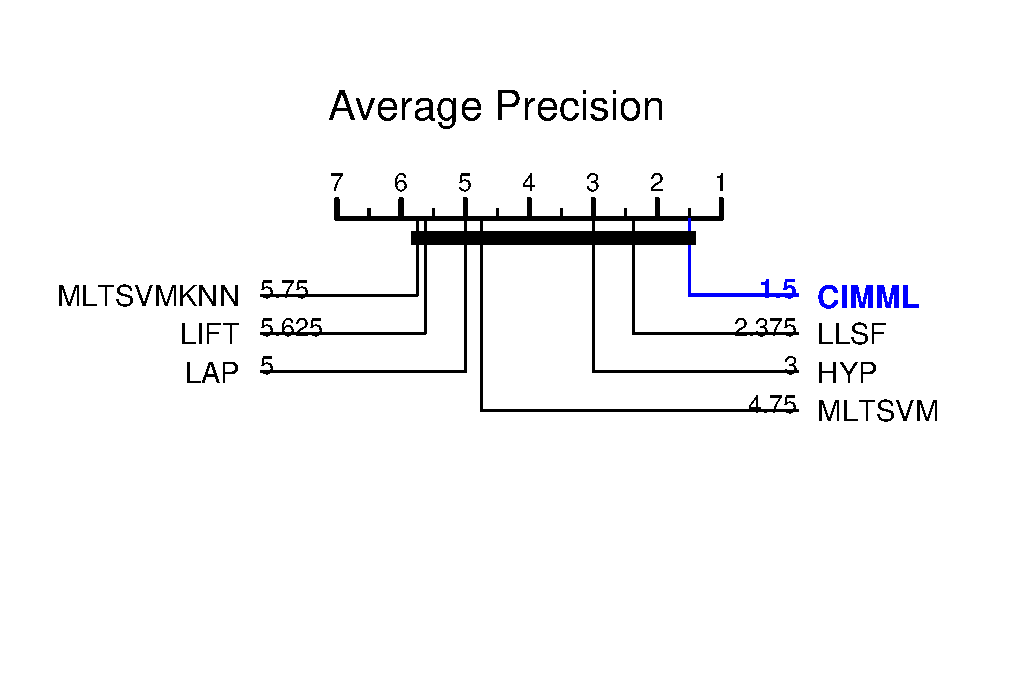
\includegraphics[width=\linewidth]{Figures/chp3/AP.eps}
        \caption*{(b) Average Precision}
        \label{figap}
    \end{minipage}

    \vspace{0.5em}

    % Row 2
    \begin{minipage}[t]{0.45\textwidth}
        \centering
        \includegraphics[width=\linewidth]{Figures/chp3/RL.eps}
        \caption*{(c) Ranking Loss}
        \label{figrl}
    \end{minipage}%
    \hspace{0.05\textwidth}
    \begin{minipage}[t]{0.45\textwidth}
        \centering
        \includegraphics[width=\linewidth]{Figures/chp3/F1.eps}
        \caption*{(d) F1}
        \label{figf1}
    \end{minipage}

    \vspace{0.5em}

    % Row 3
    \begin{minipage}[t]{0.6\textwidth}
        \centering
        \includegraphics[width=\linewidth]{Figures/chp3/AUC.eps}
        \caption*{(e) AUC}
        \label{figauc}
    \end{minipage}

    \caption{HMLLSTSVM comparison with competing algorithms using Nemenyi test, CD=2.32.}
    \label{figcd}
\end{figure*}







% Placeholder for content about HMLLSTSVM.

\newpage
\chapter{Improved Hypergraph-Laplacian-based Semi-Supervised Support Vector Machine (IHLSVM)}

\section{Hypergraph Support Vector Machine}
Laplacian Support Vector Machine assumes a pairwise association between the samples, which generally doesn't seem to hold in practice. Graph Laplacian is unable to capture multivariate and higher-order relationships between the samples. Authors in \cite{bsun2022hypergraph} express an order relationship with Hypergraph, which captures the association between two or more two vertices. Thus, the formulation of HGSVM is a quadratic programming problem given by
\begin{align}
    &\underset {\alpha \in R^n, \xi \in R^l }{\mathrm{min}} \sum_{i=1}^l \xi_i 
    + \gamma_A \alpha^T K \alpha 
    + \gamma_I \alpha^T KHK \alpha \nonumber \\
    &\text{s.t. } y_i\left(\sum_{j=1}^n \alpha_j k(x_i, x_j) + b\right) \geq 1 - \xi_i, \quad i = 1, 2, \ldots, l, \nonumber \\
    &\xi_i \geq 0, \quad i = 1, 2, \ldots, l. 
\end{align}


where \(H\) is the Laplacian regularised Hyper-Graph of the dataset as defined in \eqref{eq:15}.  The solution of the optimization, as mentioned earlier, is obtained by solving one quadratic programming problem followed by solving a system of linear equations which is not scalable.

\begin{align}
    &\underset{\beta \in R^l}{\mathrm{max}} \ \sum_{i=0}^l \beta_i - \frac{1}{2} \beta^T Q \beta \nonumber \\
    &\text{s.t.} \ \sum_{i=0}^l \beta_i y_i = 0, \nonumber \\
    &0 \leq \beta_i \leq 1, \quad i = 1, 2, \ldots, l,
\end{align}
Where 
\[
Q = Y J K \left(2\gamma_A I + 2\gamma_I K L\right)^{-1} J_L^T Y,
\]
\( I \) is the identity matrix, \( J = [I \ 0]_{l \times (l+u)} \), and \( Y = \mathrm{diag}(y_1, y_2, \ldots, y_l) \).


% Placeholder for content about IHLSVM.
\section{Improved Hypergraph Laplacian SVM (IHLSVM)}
In this section, we propose solving HGSVM, i.e., the aforementioned quadratic programming problem in primal space, by replacing hinge loss with a square-hinged loss function, which leads to solving the following unconstrained optimisation problem in the primal space.
\begin{equation} \label{eq:16}
	\begin{split}
		\underset{\alpha \in R^m,b \in R}{\mathrm{min} } & \frac{1}{2}(\sum_{i=1}^l max(1-y_i(k_i^T\alpha + b),0)^2 + \delta_A\alpha^TK\alpha + \\  
		& \delta_I(\alpha^TK + 1^Tb)HL(K\alpha + 1b))
	\end{split}
\end{equation}
Since the above optimization  is a convex problem, Newton's method is used to find the optimal solution whose complexity is $O(n^3)$. 

The graph Laplacian \(L\) carries the pairwise relationship between the training instances, while the multivariate and complex relations are carried by the Hyper-graph Laplacian matrix \(HL\). However, it is challenging to identify which representation would be optimal for the given dataset. Therefore, in this section, we define an improved Hypergraph Laplacian matrix, which is a weighted linear combination of Laplacian as well as Hypergraph Laplacian and solve it as an unconstrained optimisation problem which can be further solved in primal space using Preconditioned Conjugate Gradient method \cite{melacci2011laplacian} whose order of complexity is $O(kn^2)$, where $k$ is number of iterations and $n$ is the number of training samples.

\begin{equation} \label{eq:18}
    IHL = \lambda L + (1-\lambda) HL
\end{equation}
In the \(IHL\) matrix, \(L\) is from \eqref{manifold_learning_1} and \(H\) matrix is from \eqref{eq:18}. $\lambda$ is the hyper-parameter which work as a balancing factor between both of them. 
%such that \[\lambda_1 + \lambda_2 = 1, \] 
%\[ 0 \leq \lambda_1,\lambda_2 \leq 1\]

%%From the \eqref{eq:5}, we know
%\[
%f^* = \underset{f \in H_k }{\mathrm{arg min}} \sum_{i=1}^{l} V(x_i,y_i,f) + \delta_A||f||^2_A + \delta_I||f||^2_I 
%\]
Thus, considering squared-hinged loss function.
\[
V(x_i,y_i,f) = max(1-y_i(k_i^T\alpha + b),0)^2,
\] regulariser term as 
\(||f||^2_A = \alpha^T K \alpha\), \(|f||^2_I = \alpha^T K (IHL) K \alpha\).  IHLSVM problem would solve the following unconstrained optimisation problem



\begin{equation}\label{eq:19}
\begin{split}
   \underset{\alpha \in R^m,b \in R}{\mathrm{min}}  & \frac{1}{2}(\sum_{i=1}^l max(1-y_i(k_i^T\alpha + b),0)^2 + \delta_A\alpha^TK\alpha + \\ & \delta_I(\alpha^TK + 1^Tb)(IHL)(K\alpha + 1b)) 
\end{split}
\end{equation}


We can solve \eqref{eq:19} using the Preconditioned Conjugate Gradient (PCG) method\cite{melacci2011laplacian}. The detailed algorithm is mentioned below.

\begin{algorithm}
	\caption{Algorithm for IHLSVM}
	%\begin{algorithmic}[1]
		\renewcommand{\algorithmicrequire}{\textbf{Input:}}
		\renewcommand{\algorithmicensure}{\textbf{Output:}}
		 Dataset; $S=X\cup U=\{x_t,y_t\}_{t=1}^l\cup \{x_t\}_{t=l+1}^{l+u}$, $X$ denotes a set of $l$ labeled data, $U$ denotes set of $u$ unlabeled examples and parameters set $\sigma , \gamma_1, \gamma_2, \lambda$;
		classsifier $f(x)= sign(\sum_{i=1}^{l+u} \alpha_i^*K(x,x_i)$
		\\ \text{Initialisation}:
		\text{Calculate Graph Laplacian $L$};
		\\   \text{Calculate the Laplacian Regularised Hypergraph $HL=I-D_v^{-\frac{1}{2}}FWD_e^{-1}F^TD_v^{-\frac{1}{2}}$};\\
		 \text{Calculate Improved Hypergraph Laplacian matrix   $IHL = \lambda L + (1-\lambda) H$};\\
		 \text{Find kernel function $K(x_i,x_j)$ };\\
		 \text{Calculate $\alpha^*$ by solving primal problem  \eqref{eq:19}  by using PCG Method};
	%\end{algorithmic} 
\end{algorithm}




\section{Multi-category and Multi-label Classification}  
In semi-supervised learning, multi-class or multi-label classification is a challenging task due to the unknown geometrical structure of the data. There are many problems like speech recognition\cite{jin2017performance}, face recognition\cite{wei2011face}, and many staged diseases which are multi-class problems. There are many methods to solve multi-class like OVO(One-vs-One)\cite{galar2015drcw}, OVR(One-vs-Rest)\cite{rifkin2004defense} or DAG for multi-class classification\cite{platt1999large}, and Binary Relevance(BR)\cite{zhang2018binary} for multi-label classification. We have adopted the OVR classification strategy for multiclass and binary relevance for multi-label classification for experiment purposes.

\section{Experiments and Results}
We ran a large set of experiments to analyse the Improved Hypergraph Laplacian Support Vector Machine (IHLSVM) proposed solution strategies and compared them with other algorithms like LapSVM and HGSVM. In this section, we discuss data sets, our experimental protocol and the details of parameter selection strategy. We perform numerical experiments on UCI datasets. All the experiments are performed in MATLAB R2023a on a PC with AMD Ryzen 7 5800U with Radeon Graphics 1.90 GHz and 8GB RAM.

\subsection{UCI Datasets}
We ran tests on 12 UCI \footnote{https://archive.ics.uci.edu/} benchmark datasets to look into the classification performance of our proposed approach with the square-hinge loss version of LapSVM and HGSVM. Table \ref{table:1} presents specifics of the 12 UCI benchmark datasets and multilabel datasets \footnote{https://www.uco.es/kdis/mllresources}. Every dataset is standardised with mean zero and staa mean zero and a standard deviation of ndard deviation 1.


\begin{table}[htbp]
\caption{UCI datasets}
\begin{center}
\begin{tabular}{|l|c|c|c|}
\hline
\textbf{Dataset } & \textbf{ Size }& \textbf{ Features }& \textbf{ Classes } \\
\hline
Australian & 690 & 14 & 2 \\ 
 Breast Cancer & 277 & 9 & 2 \\
 CMC & 1473 & 9 & 2 \\
 German & 1000 & 24 & 2 \\
 Hearts & 270 & 13 & 2 \\
 Ionosphere & 351 & 34 & 2 \\
 WDBC & 569 & 30 & 2 \\
 Ecoli & 3186 & 3 & 3 \\
 Dna & 3186  & 180 & 3 \\
 Glass & 214 & 9 & 7 \\
 Iris & 150 & 4 & 3 \\
 Wine & 178 & 13 & 3 \\
\hline
\end{tabular}
\label{table:1}
\end{center}
\end{table}

\subsubsection{Results for Binary Classification.}
 We have compared IHLSVM with square-hinge loss version of LapSVM and HGSVM, on seven  UCI binary datasets. We have used 10-fold cross-validation to report the accuracy of models, where two regularisation parameters have range \( \{10^{-6},10^{-5},...,1,10,100\} \) and kernel parameters for RBF have the range \([0,1]\).  Table  \ref{binary} %and Fig.\ref{fig:2} 
report the mean accuracy with standard deviation. We can observe that the classification performance of our proposed IHLSVM is better than that of the other two methods on all binary datasets. In addition, we investigate the classification performances of IHLSVM under \(0\%, 10 \%, 20 \%, 30 \%, 40, 50 \%, 60 \%, 70 \% \) unlabelled data used while training.

%\begin{figure*}[htbp]
%\centerline{\includegraphics[scale=0.4]{binary_results.png}}
%\caption{Results for Binary classification}
%\label{fig:2}
%\end{figure*}

\begin{table*}[htbp]
	\caption{Classification Accuracy Results for Binary Datasets}
\small
	\centering
	\setlength\tabcolsep{0pt}
	\begin{tabular*}{\linewidth}{@{\extracolsep{\fill}} |c|clll| }
		\hline
		\textbf{ Dataset} & \textbf{Unlabelled } & \textbf{LapSVM} & \textbf{HGSVM} & \textbf{IHLSVM } \\ \hline
		~ & 0\% & 80.29 $\pm$6.70\%  & 80.00 $\pm$6.62\% & \textbf{80.87 $\pm$6.10\% }  \\ 
		~ & 10\% & 81.01 $\pm$5.48\%  & 80.87 $\pm$5.33\%  & \textbf{81.16 $\pm$5.63\% }  \\ 
            ~ & 20\% & 82.46 \(\pm\)5.65\%  & 82.46 \(\pm\)5.65\%  & \textbf{82.75 \(\pm\)5.53\%} \\
            \textbf{ Australian }  & 30\% & 80.87 $\pm$5.19\% & 81.01 $\pm$5.18\%  & \textbf{81.45 $\pm$4.20\%} \\ 
		~ & 50\% & 81.30 $\pm$4.50\%  & 81.30 $\pm$4.50\%  & \textbf{81.45 $\pm$4.62\%}  \\ 
            ~ & 60\% & 79.71 \(\pm\)4.83\%  & 81.30 \(\pm\)4.50\%  & \textbf{81.88 \(\pm\)4.39\%} \\
            ~ & 70\% & 86.36 \(\pm\)1.17\%  & 86.33 \(\pm\)1.20\%  & \textbf{86.49 \(\pm\)1.12\%} \\ 
		\hline
		~ & 0\% & 71.90 $\pm$4.70\% & 72.10 $\pm$4.43\%  & \textbf{72.50 $\pm$4.43\%}  \\ 
		~ & 10\% & 71.30 $\pm$4.42\% & 71.30 $\pm$4.57\% & \textbf{71.80 $\pm$4.44\%} \\ 
            ~ & 20\% & 71.70 \(\pm\)4.37\%  & 71.30 \(\pm\)4.79\% &  \textbf{71.80 \(\pm\)3.82\%} \\
		\textbf{ German } & 30\% & 72.00 $\pm$3.50\%  & 72.00 $\pm$3.83\% & \textbf{72.20 $\pm$2.97\%}  \\ 
		~ & 50\% & 70.80 $\pm$5.35\%  & 71.00 $\pm$4.99\%  & \textbf{71.10 $\pm$4.89\%}  \\ 
            ~ & 60\% & 70.10 \(\pm\)4.61\%  & 70.10 \(\pm\)4.61\% &  \textbf{70.40 \(\pm\)4.45\%} \\
            ~ & 70\% & 71.60 \(\pm\)4.30\%  & 71.80 \(\pm\)4.59\% &  \textbf{71.90 \(\pm\)4.77\%} \\ 
		\hline
		~ & 0\% & 94.32 $\pm$3.24\%  & 94.31 $\pm$3.28\%  & \textbf{94.60 $\pm$3.36\%} \\
		~ & 10\% & 94.02 $\pm$3.68\% & \textbf{94.02 $\pm$3.68\%}  & 93.74 $\pm$3.75\% \\ 
            ~ & 20\% & 93.47 \(\pm\)4.98\% & 94.04 \(\pm\) 5.23\%  &  \textbf{93.75 \(\pm\)5.11\%} \\
		\textbf{ Ionosphere } & 30\% & 92.04 $\pm$3.69\% & 92.04 $\pm$3.69\%  & \textbf{92.33 $\pm$3.75\%} \\ 
		~ & 50\% & 92.03 $\pm$4.19\% & 92.03 $\pm$4.60\%  & \textbf{92.32 $\pm$4.45\%}  \\
            ~ & 60\% & 90.33 \(\pm\)4.26\% & 90.33 \(\pm\)4.04\%  &  \textbf{90.90 \(\pm\)3.70\%} \\
            ~ & 70\% & 64.95 \(\pm\)7.64\% & 64.95 \(\pm\)7.64\%  &  \textbf{65.24 \(\pm\)7.61\%} \\
		\hline
		~ & 0\% & 70.74 $\pm$5.80\%  & \textbf{70.74 $\pm$5.80\%}  & 71.10 $\pm$5.71\%  \\ 
		~ & 10\% & 71.14 $\pm$6.20\%  & 71.14 $\pm$6.20\% & \textbf{71.85 $\pm$6.19\%}  \\ 
            ~ & 20\% & 65.36 \(\pm\)7.33\% & 65.56 \(\pm\)7.33\% & \textbf{66.43 \(\pm\)8.09\%} \\
		 \textbf{ Breast Cancer } & 30\% & 69.70 $\pm$9.04\% & 63.92 $\pm$7.91\% & \textbf{70.04 $\pm$7.73\%}  \\ 
		~ & 50\% & 71.85 $\pm$3.64\%  & 67.87 $\pm$7.72\% & \textbf{72.21 $\pm$4.13\%}  \\ 
            ~ & 60\% & 67.53 \(\pm\)5.54\% & 64.47 \(\pm\)7.58\% & \textbf{67.87 \(\pm\)6.69\%} \\
            ~ & 70\% & 72.91 \(\pm\)6.04\% & 67.50 \(\pm\)5.91\% & \textbf{72.94 \(\pm\)5.64\%} \\
		\hline
		~ & 0\% & 66.05 $\pm$4.04\%  & 65.57 $\pm$4.38\%  & \textbf{66.12 $\pm$3.84\%} \\ 
		~ & 10\% & 66.46 $\pm$3.42\%  & 66.19 $\pm$3.48\%  & \textbf{66.52 $\pm$3.90\%}  \\
            ~ & 20\% & 64.56 \(\pm\)2.56 \% & 65.78 \(\pm\)2.53\%  & \textbf{66.19 \(\pm\)3.17\%} \\ 
		\textbf{ CMC } & 30\% & 65.92 $\pm$3.72\%  & 65.37 $\pm$2.75\% & \textbf{66.05 $\pm$3.21\%} \\ 
		~ & 50\% & 65.17 $\pm$4.15\%  & 65.24 $\pm$3.84\%  & \textbf{65.44 $\pm$4.81\%}  \\ 
            ~ & 60 \% & 62.65 \(\pm\)4.49\%  & 62.58 \(\pm\)5.48\%  & \textbf{63.40 \(\pm\)4.43\%} \\
            ~ & 70 \% & 61.78 \(\pm\)3.81\%  & 60.82 \(\pm\)4.41\%  & \textbf{62.05 \(\pm\)3.73\%} \\
		\hline
		~ & 0\% & 76.30 $\pm$8.04\%  & 75.19 $\pm$6.99\%  & \textbf{77.41 $\pm$7.29\%} \\
		~ & 10\% & 76.67 $\pm$8.56\%  & 75.93 $\pm$8.42\%  & \textbf{78.89 $\pm$8.38\%} \\ 
            ~ & 20\% & 77.78 \(\pm\)9.56\%  & 76.67 \(\pm\)12.10\% & \textbf{78.89 \(\pm\)8.74\%} \\ 
		\textbf{ Hearts-statlog } & 30\% & 79.26 $\pm$5.58\% & 78.52 $\pm$9.53\% & \textbf{80.37 $\pm$6.54\%}  \\ 
		~ & 50\% & 80.00 $\pm$6.10\%  & 80.37 $\pm$5.80\%  & \textbf{81.48 $\pm$7.20\%}  \\ 
            ~ & 60\% & 80.00 \(\pm\)8.04\%  & 80.37 \(\pm\)8.91\%  & \textbf{81.11 \(\pm\)8.27\% } \\
            ~ & 70\% & 81.11 \(\pm\)7.90\%  & 80.00 \(\pm\)8.94\%  & \textbf{81.48 \(\pm\)7.20\%} \\
		\hline
		~ & 0\% & 96.14 $\pm$3.77\% & 95.09 $\pm$3.39\%  & \textbf{96.32 $\pm$4.09\%} \\ 
		~ & 10\% & 96.66 $\pm$3.14\%  & 95.08 $\pm$3.18\%  & \textbf{96.84 $\pm$2.96\%}  \\ 
            ~ & 20\% & 96.49 \(\pm\)2.61\%  & 96.31 \(\pm\)2.67\% & \textbf{96.66 \(\pm\)2.40\%} \\ 
		\textbf{ WDBC } & 30\% & 96.66 $\pm$2.40\%  & 96.49 $\pm$1.85\% & \textbf{96.84 $\pm$1.61\%} \\ 
		~ & 50\% & 96.32 $\pm$2.67\%  & 96.49 $\pm$2.48\%  & \textbf{97.02 $\pm$2.20\%} \\
            ~ & 60\% & 96.49 \(\pm\)3.20\%  & 96.32 \(\pm\)3.14\% & \textbf{96.67 \(\pm\)3.14\%} \\
            ~ & 70\% & 96.14 \(\pm\)3.39\%  & 96.14 \(\pm\)2.96\% & \textbf{96.32 \(\pm\)3.45\%} \\
		\hline
	\end{tabular*}
	\label{binary}
\end{table*}



\subsubsection{Results for Multi‑class Classification}
We investigate the classification performance of our proposed method on five UCI multi-class datasets and have evaluate its performance on Fashion MNIST data. We have used the OVR\cite{rifkin2004defense} strategy and compared it with the square-hinge loss version of LapSVM and HGSVM. We are using 10-fold cross-validation to report the classification accuracy.
Each experiment is also repeated ten times. Table ~\ref{multi} reports the mean accuracy and its standard deviation. We can observe that the classification performance of our proposed IHLSVM is better than that of the other two methods on all multi-class datasets. In addition, we investigate the classification performances of IHLSVM under \(0 \%, 10 \%, 20 \%, 30 \% \) unlabelled data used while training. Fashion-MNIST \footnote{https://tech.zalando.comt} is a dataset of Zalando's article images—consisting of a training set of 60,000 examples and a test set of 10,000 examples. Each example is a 28x28 grayscale image associated with a label from 10 classes. Zalando intends Fashion-MNIST to be a direct drop-in replacement for the original MNIST dataset for benchmarking machine learning algorithms. It shares the same image size and structure of training and testing splits. We investigate the classification performances of IHLSVM under \(0 \%, 10 \%, 20 \%, 30 \% 40 \%, 50 \%\) unlabelled data in the training dataset. Mean and standard deviation are reported in Table \ref{table:20} and fig. \ref{fig:4} illustrates the performance for various percentages of unlabelled data. \ref{sens_binary} and \ref{sens_multi} reports an ablation study to discuss the performance of the proposed algorithm (IHLSVM) for different values of hyperparameters, i.e. kernel parameter ($\sigma$), $\delta_A$, $\delta_I$, $\lambda$.

\begin{table*}[!ht]
    \caption{Classification Accuracy Results for Multi-class Datasets}
    \centering
    \setlength\tabcolsep{8pt} % Adjust column separation for better spacing
    \renewcommand{\arraystretch}{1.2} % Adjust row spacing for readability
    \begin{tabular*}{\linewidth}{@{\extracolsep{\fill}}|c|c|c|c|c|}
        \hline
        \textbf{Dataset} & \textbf{Unlabelled Percentage} & \textbf{LapSVM} & \textbf{HGSVM} & \textbf{IHLSVM} \\
        \hline
        \multirow{4}{*}{\textbf{Ecoli}} 
        & 0\%  & 85.71 $\pm$ 3.76\% & 85.71 $\pm$ 3.77\% & \textbf{86.01 $\pm$ 3.92\%} \\ 
        & 10\% & 85.11 $\pm$ 3.84\% & 84.52 $\pm$ 3.77\% & \textbf{85.71 $\pm$ 3.77\%} \\ 
        & 20\% & 85.71 $\pm$ 3.90\% & 85.40 $\pm$ 4.68\% & \textbf{86.30 $\pm$ 4.30\%} \\ 
        & 30\% & 81.23 $\pm$ 5.88\% & 81.23 $\pm$ 6.51\% & \textbf{83.32 $\pm$ 3.76\%} \\ 
        \hline
        \multirow{4}{*}{\textbf{Iris}} 
        & 0\%  & 92.00 $\pm$ 5.06\% & 93.33 $\pm$ 5.27\% & \textbf{94.67 $\pm$ 5.06\%} \\ 
        & 10\% & 92.67 $\pm$ 5.48\% & 91.33 $\pm$ 9.60\% & \textbf{95.33 $\pm$ 3.80\%} \\ 
        & 20\% & 92.67 $\pm$ 10.90\% & 90.00 $\pm$ 8.16\% & \textbf{94.67 $\pm$ 5.06\%} \\ 
        & 30\% & 92.67 $\pm$ 7.96\% & 94.00 $\pm$ 4.35\% & \textbf{94.67 $\pm$ 4.47\%} \\ 
        \hline
        \multirow{4}{*}{\textbf{Wine}} 
        & 0\%  & 98.30 $\pm$ 1.55\% & 98.32 $\pm$ 1.54\% & \textbf{98.87 $\pm$ 1.54\%} \\ 
        & 10\% & 97.73 $\pm$ 2.39\% & 97.75 $\pm$ 1.26\% & \textbf{98.30 $\pm$ 1.55\%} \\ 
        & 20\% & 98.86 $\pm$ 1.56\% & 98.87 $\pm$ 1.54\% & \textbf{99.43 $\pm$ 1.28\%} \\ 
        & 30\% & 93.81 $\pm$ 2.37\% & 93.25 $\pm$ 1.56\% & \textbf{93.83 $\pm$ 1.21\%} \\ 
        \hline
        \multirow{4}{*}{\textbf{Glass}} 
        & 0\%  & 66.36 $\pm$ 7.80\% & 66.38 $\pm$ 6.97\% & \textbf{67.30 $\pm$ 8.66\%} \\ 
        & 10\% & 64.99 $\pm$ 5.92\% & 64.03 $\pm$ 3.74\% & \textbf{65.46 $\pm$ 5.80\%} \\ 
        & 20\% & 58.89 $\pm$ 8.55\% & 57.96 $\pm$ 8.75\% & \textbf{60.29 $\pm$ 8.81\%} \\ 
        & 30\% & 53.28 $\pm$ 6.90\% & 52.34 $\pm$ 6.26\% & \textbf{53.73 $\pm$ 6.28\%} \\ 
        \hline
        \multirow{4}{*}{\textbf{DNA}} 
        & 0\%  & 50.25 $\pm$ 1.95\% & 50.22 $\pm$ 1.96\% & \textbf{50.38 $\pm$ 1.93\%} \\ 
        & 10\% & 50.22 $\pm$ 1.90\% & 50.16 $\pm$ 1.72\% & \textbf{50.25 $\pm$ 1.74\%} \\ 
        & 20\% & 50.66 $\pm$ 1.97\% & 50.56 $\pm$ 1.78\% & \textbf{50.75 $\pm$ 1.87\%} \\ 
        & 30\% & 51.07 $\pm$ 1.84\% & 51.13 $\pm$ 1.75\% & \textbf{51.22 $\pm$ 1.66\%} \\ 
        \hline
    \end{tabular*}
    \label{multi}
\end{table*}



\begin{table}[htbp]
	\caption{Comparison of Results for MNIST Fashion}
	\begin{center}
		\begin{tabular}{|c|c|c|c|}
			\hline
			\textbf{Unlabelled } & \textbf{ LapSVM }& \textbf{ HGSVM }& \textbf{ IHLSVM } \\
			\hline
			0  \% & 76.57\(\pm\) 0.79 & 	76.48\(\pm\) 1.41 &	\textbf{76.89\(\pm\) 0.84} \\
			10 \% & \textbf{76.45\(\pm\) 0.84} & 	75.88\(\pm\) 0.81 & 	76.41\(\pm\) 0.72 \\
			20 \% & 75.07\(\pm\) 0.98 & 	75.38\(\pm\) 1.18 &	\textbf{75.43\(\pm\) 1.10} \\
			30 \% & 74.55\(\pm\) 1.56 & 	\textbf{74.75\(\pm\) 0.52} &	74.70\(\pm\) 1.41 \\
			40 \% & 73.91\(\pm\) 0.96 & 	73.21\(\pm\) 1.82 & 	\textbf{74.16\(\pm\) 0.98} \\
			50 \% & 72.62\(\pm\) 1.28 & 	71.82\(\pm\) 1.23 &	\textbf{72.88\(\pm\) 1.25} \\
			\hline
		\end{tabular}
		\label{table:20}
	\end{center}
\end{table}

\begin{figure}
	\centerline{\includegraphics[scale=0.4]{Figures/chp4/mnist_fashion.png}}
	\caption{Results for MNIST Fashion}
	\label{fig:4}
\end{figure}

\begin{table}[htbp]
	\caption{Description of Multi-label Datasets}
	\begin{center}
		\begin{tabular}{|l|c|c|c|c|c|}
			\hline
			\textbf{Dataset } & \textbf{ Instances }& \textbf{ Features }& \textbf{ Labels }& \textbf{ Card } & \textbf{ Domain } \\
			\hline
			Birds & 645 &260 &19 & 1.014& Audio\\
			CAL500 & 502& 68& 174& 26.044& Music\\
			Emotions  & 593& 72& 6& 1.868& Music\\
			Flags & 194& 19& 7& 3.392& Image\\
			Image & 2000& 294& 5& 1.236& Image\\
			Enron & 1702  & 1001 & 53 & 3.378& text \\
			\hline
		\end{tabular}
		\label{table:14}
	\end{center}
\end{table}
  \begin{figure*}[t!] % Use 'H' for precise location if needed
    \centering
    % First Row
    \begin{minipage}[t]{0.5\textwidth}
        \centering
        \includegraphics[width=0.9\linewidth]{Figures/chp4/ablation/aus_sigma.pdf}
        % \caption*{Kernel Sensitivity Analysis for Wine Dataset}
    \end{minipage}%
    \begin{minipage}[t]{0.5\textwidth}
        \centering
        \includegraphics[width=0.9\linewidth]{Figures/chp4/ablation/german_sigma.pdf}
        % \caption*{Kernel Sensitivity Analysis for German Dataset}
        \label{fig:german_kernel}
    \end{minipage}
    \vspace{0.5cm} % Add vertical spacing between rows

    % Second Row
    \begin{minipage}[t]{0.5\textwidth}
        \centering
        \includegraphics[width=1.0\linewidth]{Figures/chp4/ablation/aus_lambda.pdf}
        % \caption*{Lambda Sensitivity Analysis for Wine Dataset}
        \label{fig:aus_lambda}
    \end{minipage}%
    \begin{minipage}[t]{0.5\textwidth}
        \centering
        \includegraphics[width=0.9\linewidth]{Figures/chp4/ablation/germany_lambda.pdf}
        % \caption*{Lambda Sensitivity Analysis for German Dataset}
        \label{fig:german_lambda}
    \end{minipage}
    \vspace{0.5cm}

    % Third Row (Two Columns)
    \begin{minipage}[t]{0.5\textwidth}
        \centering
        \includegraphics[width=0.9\linewidth]{Figures/chp4/ablation/aus_gamma.pdf}
        % \caption*{$\delta_A$ and $\delta_I$ Sensitivity Analysis for Wine Dataset}
        \label{fig:aus_gamma}
    \end{minipage}%
    \begin{minipage}[t]{0.5\textwidth}
        \centering
        \includegraphics[width=0.9\linewidth]{Figures/chp4/ablation/german_gamma.pdf}
        % \caption*{$\delta_A$ and $\delta_I$ Sensitivity Analysis for German Dataset}
        \label{fig:german_gamma}
    \end{minipage}

    \caption{Sensitivity Analysis for binary datasets German and Austrlian.}
    \label{sens_binary}
\end{figure*}

\begin{figure*}[t!] % Use 'H' for precise location if needed
    \centering
    % First Row
    \begin{minipage}[t]{0.5\textwidth}
        \centering
        \includegraphics[width=0.9\linewidth]{Figures/chp4/ablation/ecoli_sigma.pdf}
        % \caption*{Kernel Sensitivity Analysis for Ecoli Dataset}
    \end{minipage}%
    \begin{minipage}[t]{0.5\textwidth}
        \centering
        \includegraphics[width=0.9\linewidth]{Figures/chp4/ablation/wine_sigma.pdf}
        % \caption*{Kernel Sensitivity Analysis for Australian Dataset}
        \label{fig:wine_kernel}
    \end{minipage}
    \vspace{0.5cm} % Add vertical spacing between rows

    % Second Row
    \begin{minipage}[t]{0.5\textwidth}
        \centering
        \includegraphics[width=1.0\linewidth]{Figures/chp4/ablation/ecoli_lambda.pdf}
        % \caption*{Lambda Sensitivity Analysis for Ecoli Dataset}
        \label{fig:ecoli_lambda}
    \end{minipage}%
    \begin{minipage}[t]{0.5\textwidth}
        \centering
        \includegraphics[width=0.9\linewidth]{Figures/chp4/ablation/wine_lambda.pdf}
        % \caption*{Lambda Sensitivity Analysis for Australian Dataset}
        \label{fig:wine_lambda}
    \end{minipage}
    \vspace{0.5cm}

    % Third Row (Two Columns)
    \begin{minipage}[t]{0.5\textwidth}
        \centering
        \includegraphics[width=0.9\linewidth]{Figures/chp4/ablation/ecoli_gamma.pdf}
        % \caption*{$\delta_A$ and $\delta_I$ Sensitivity Analysis for Eoli Dataset}
        \label{fig:ecoli_gamma}
    \end{minipage}%
    \begin{minipage}[t]{0.5\textwidth}
        \centering
        \includegraphics[width=0.9\linewidth]{Figures/chp4/ablation/wine_gamma.pdf}
        % \caption*{$\delta_A$ and $\delta_I$ Sensitivity Analysis for Australian Dataset}
        \label{fig:wine_gamma}
    \end{minipage}

    \caption{Sensitivity Analysis for multi-category datasets Ecoli and Wine}
    \label{sens_multi}
\end{figure*}
 

\subsection{Results for Multi-label Classification} We investigate the classification performance of our proposed method along with the square hinge loss version of LapSVM and HGSVM on four multi-label datasets, i.e. Birds, Cal500, Flags, and Enron discussed in  Table \ref{table:14}. We have used the five evaluation criteria, Hamming Loss, Average Precision, Ranking Loss, AUC and F1 Score,  to compare the performance of multi-label classification algorithms and results are discussed in Table \ref{tabel_ml_start} - Table \ref{tabel_ml_end} for performances of IHLSVM under \(0 \%, 10  \%, 30, 50 \%\) unlabelled data used while training. 
In Figure \ref{sens_binary} and Figure \ref{sens_multi}, we have reported the Nemenyi Test\cite{demvsar2006statistical} in Figure \ref{figcd_IHLSVM} for comparing the performance of IHLSVM with the other two algorithms on five metrics. 
% \begin{figure*}[htp]
% \centering
% %\begin{minipage}[t]{0.5\linewidth}
% \includegraphics[width=5in,height=3in]{multi_class_results.png}
% \caption{Results for Multiclass classification}
% \label{fig:3}
% \parbox{6.5cm}{\small \hspace{1.5cm} }
% %\end{minipage}
% \end{figure*}



% \begin{table}
% 	\caption{Comparison of Results on Multi-label Datasets}
% 	\centering
% 	\setlength\tabcolsep{0pt}
% 	\begin{tabular*}{\linewidth}{@{\extracolsep{\fill}} |c|lrrc||rrc|}
% 		\hline        
% 		\textbf{Dataset} & \textbf{Metric }  & \textbf{LapSVM }  & \textbf{HGSVM } & \textbf{IHLSVM }& \textbf{LapSVM }  & \textbf{HGSVM } & \textbf{IHLSVM } \\ 
% 		Unlabelled& ~ & ~ & 0\% & ~ & ~ & 10\% & ~ \\ \hline 
% 		~ & HL$(\downarrow)$ & 0.0458 & 0.0468 & \textbf{0.0452} & 0.0458 & 0.0474 & \textbf{0.0455} \\ 
% 		~ & F1$(\uparrow)$ & 0.6158 & 0.6095 & \textbf{0.62} & 0.6097 & 0.5927 & \textbf{0.6131} \\ 
% 		Birds & AP$(\uparrow)$ & 0.1429 & 0.1524 & 0.1429 & 0.1167 & \textbf{0.1362} & 0.1262 \\ 
% 		~ & RL$(\downarrow)$ & 0.7675 & 0.7669 & \textbf{0.7632} & 0.7908 & 0.8069 & \textbf{0.7901} \\ 
% 		~ & AUC$(\uparrow)$ & 0.6726 & 0.6731 & \textbf{0.6743} & \textbf{0.6494} & 0.6382 & 0.6481 \\ 
% 		\hline 
% 		~ & HL$(\downarrow)$ & 0.3084 & 0.3077 & \textbf{0.3062} & 0.3056 & 0.3027 & \textbf{0.3019} \\ 
% 		~ & F1$(\uparrow)$ & 0.664 & 0.6641 & \textbf{0.6671} & 0.6768 & 0.6794 & \textbf{0.6821} \\ 
% 		Flags & AP$(\uparrow)$ & 0.0571 & 0.0571 & \textbf{0.0571} & 0.1143 & 0.1143 & \textbf{0.1143} \\ 
% 		~ & RL$(\downarrow)$ & 0.7014 & \textbf{0.6979} & 0.6983 & 0.6881 & 0.6849 & \textbf{0.6803} \\ 
% 		~ & AUC$(\uparrow)$ & 0.5773 & \textbf{0.5789} & 0.5787 & 0.5928 & 0.5952 & \textbf{0.5987} \\ 
% 		\hline 
% 		~ & HL$(\downarrow)$ & \textbf{0.1386} & 0.1388 & 0.1387 & 0.1381 & 0.138 & \textbf{0.138} \\ 
% 		~ & F1$(\uparrow)$ & 0.3086 & \textbf{0.3101} & 0.3096 & 0.3054 & \textbf{0.3072} & 0.3071 \\ 
% 		Cal500 & AP$(\uparrow)$ & 0.0959 & 0.1055 & \textbf{0.1055} & 0.1243 & \textbf{0.1339} & 0.1255 \\ 
% 		~ & RL$(\downarrow)$ & 0.9901 & \textbf{0.9886} & 0.9892 & 0.991 & \textbf{0.9898} & 0.9902 \\ 
% 		~ & AUC$(\uparrow)$ & 0.4712 & \textbf{0.4715} & 0.4714 & 0.4718 & \textbf{0.4726} & 0.4725 \\ 
% 		\hline 
% 		~ & HL$(\downarrow)$ & 0.0583 & 0.0585 & \textbf{0.0583} & 0.0586 & 0.058 & \textbf{0.0574} \\ 
% 		~ & F1$(\uparrow)$ & 0.4266 & \textbf{0.4282} & 0.4272 & 0.3592 & 0.4405 & \textbf{0.441} \\ 
% 		Enron & AP$(\uparrow)$ & 0.2412 & 0.2538 & \textbf{0.2412} & \textbf{0.1764} & 0.1724 & 0.1724 \\ 
% 		~ & RL$(\downarrow)$ & 0.9304 & 0.9295 & \textbf{0.9295} & 0.9311 & 0.9291 & \textbf{0.9289} \\ 
% 		~ & AUC$(\uparrow)$ & \textbf{0.486} & 0.4854 & 0.4858 & 0.4868 & 0.4871 & \textbf{0.4889} \\ 
% 		\hline
% 	\end{tabular*}
% \label{multilabel21}
% \end{table}

% \begin{table}
% 	\caption{Comparison of results on Multilabel datasets}
% 	\centering
% 	\setlength\tabcolsep{0pt}
% 	\begin{tabular*}{\linewidth}{@{\extracolsep{\fill}} |c|lrrc||rrc| }
% 		\hline
% 		\textbf{Dataset} & \textbf{Metric} & \textbf{LapSVM} & \textbf{HGSVM} & \textbf{IHLSVM} & \textbf{LapSVM} & \textbf{HGSVM} & \textbf{IHLSVM } \\ 
% 		Unlabelled & ~ & ~ & 30\% & ~ & ~ & 50\% & ~ \\ \hline
% 		~ & HL$(\downarrow)$ & 0.0477 & 0.048 & \textbf{0.047} & 0.0531 & 0.0537 & \textbf{0.053} \\ 
% 		~ & F1$(\uparrow)$ & 0.5519 & 0.5581 & \textbf{0.5635} & \textbf{0.498} & 0.4945 & 0.4959 \\ 
% 		Birds & AP$(\uparrow)$ & 0.0581 & \textbf{0.0771} & 0.0386 & \textbf{0.0776} & 0.0781 & 0.0581 \\ 
% 		~ & RL$(\downarrow)$ & 0.8153 & 0.8353 & \textbf{0.8137} & \textbf{0.8432} & 0.8698 & 0.8486 \\ 
% 		~ & AUC$(\uparrow)$ & 0.624 & 0.6201 & \textbf{0.6265} & \textbf{0.5873} & 0.5801 & 0.5854 \\ 
% 		\hline
% 		~ & HL$(\downarrow)$ & 0.3175 & 0.3168 & \textbf{0.3146} & 0.318 & 0.3225 & \textbf{0.3158} \\ 
% 		~ & F1$(\uparrow)$ & 0.6672 & 0.6689 & \textbf{0.6705} & 0.6713 & 0.6671 & \textbf{0.6748} \\ 
% 		Flags & AP$(\uparrow)$ & 0.0571 & 0.0571 & \textbf{0.0571} & 0.0286 & 0.0286 & \textbf{0.0286} \\ 
% 		~ & RL$(\downarrow)$ & 0.7097 & 0.7084 & \textbf{0.7055} & 0.7189 & 0.727 & \textbf{0.7175} \\ 
% 		~ & AUC$(\uparrow)$ & 0.5774 & 0.578 & \textbf{0.5792} & 0.5745 & 0.5701 & \textbf{0.5759} \\ 
% 		\hline
% 		~ & HL$(\downarrow)$ & \textbf{0.139} & 0.1395 & 0.1395 & 0.14 & \textbf{0.1394} & 0.1401 \\ 
% 		~ & F1$(\uparrow)$ & 0.3101 & 0.3097 & \textbf{0.311} & 0.3064 & 0.308 & \textbf{0.3091} \\ 
% 		Cal500 & AP$(\uparrow)$ & 0.0754 & \textbf{0.0827} & 0.079 & \textbf{0.0685} & 0.0553 & 0.0649 \\ 
% 		~ & RL$(\downarrow)$ & 0.9916 & 0.9912 & \textbf{0.9909} & 0.9919 & 0.9923 & \textbf{0.9915} \\ 
% 		~ & AUC$(\uparrow)$ & \textbf{0.4737} & 0.4731 & 0.4733 & 0.4752 & \textbf{0.4764} & 0.4755 \\ 
% 		\hline
% 		~ & HL$(\downarrow)$ & 0.0583 & 0.0587 & \textbf{0.0583} & 0.0611 & \textbf{0.0584} & 0.0586 \\ 
% 		~ & F1$(\uparrow)$ & 0.3252 & \textbf{0.4251} & 0.3258 & 0.1326 & \textbf{0.3815} & 0.2721 \\ 
% 		Enron & AP$(\uparrow)$ & 0.216 & \textbf{0.2161} & 0.2119 & 0.1341 & 0.1425 & \textbf{0.1425} \\ 
% 		~ & RL$(\downarrow)$ & 0.942 & 0.9424 & \textbf{0.9418} & 0.9478 & 0.9459 & \textbf{0.943}8 \\ 
% 		~ & AUC$(\uparrow)$ & \textbf{0.4863} & 0.4848 & 0.4862 & 0.4694 & 0.4745 & \textbf{0.476} \\ 
% 		\hline
% 	\end{tabular*}
% \label{multilabel22}
% \end{table}




% \begin{table}[htbp]
% 	\caption{Results of Multi-label Dataset Birds}
%     \tiny
% 	\begin{center}
% 		\begin{tabular}{|c|c|c|c|c|}
% 			\hline
% 			\textbf{Unlabelled} &\textbf{Metric}& \textbf{LapSVM}& \textbf{HGSVM}& \textbf{IHLSVM}\\
% 			\hline
			
% 			& HL(\(\downarrow \)) &  0.0458  & 	0.0468          & 	\textbf{0.0452}\\
% 			& F1(\(\uparrow\))    &  0.61581 & 	0.6095          & 	\textbf{0.6200}\\
% 			0\(\%\) & AP(\(\uparrow\))    &  0.1429  & 	\textbf{0.1524} & 	0.1429\\
% 			& RL(\(\downarrow \)) &  0.7675  & 	0.7669          & 	\textbf{0.7632}\\
% 			& AUC(\(\uparrow \))  &  0.6726  & 	0.6731          & 	\textbf{0.6743}\\
% 			\hline
% 			& HL(\(\downarrow \))  &  0.0458  &	 0.0474  &	\textbf{0.0455}\\
% 			& F1(\(\uparrow\))     &  0.6097  &	 0.5927  &	\textbf{0.6131}\\
% 			10\(\%\) & AP(\(\uparrow\))     &  0.1167  &  \textbf{0.1362}  &	 0.1262\\
% 			& RL(\(\downarrow \))  &  0.7908  &	 0.8069  &	\textbf{0.7901}\\
% 			& AUC(\(\uparrow \))   &  \textbf{0.6494}  &	 0.6382  &	0.6481\\
% 			\hline
			
			
% 			& HL(\(\downarrow \))  &  0.0477  &  0.0480  &	\textbf{0.0470}  \\
% 			& F1(\(\uparrow\))     &  0.5519  &  0.5581  &	\textbf{0.5635}  \\
% 			30\(\%\)& AP(\(\uparrow\))     &  0.0581  &  \textbf{0.0771}  &	0.0386  \\
% 			& RL(\(\downarrow \))  &  0.8153  &  0.8353  &	\textbf{0.8137}  \\
% 			& AUC(\(\uparrow \))   &  0.6240  &  0.6201  &	\textbf{0.6265}  \\
% 			\hline
% 			& HL(\(\downarrow \))  &  0.0531       &  0.0537      &	\textbf{0.0530}\\
% 			& F1(\(\uparrow\))     &  \textbf{0.4980}       &  0.4945      &	0.4959\\
% 			50\(\%\) & AP(\(\uparrow\))     &  \textbf{0.0776}       &  0.0781      & 0.0581\\
% 			& RL(\(\downarrow \))  &  \textbf{0.8432}       &  0.8698      & 0.8486\\
% 			& AUC(\(\uparrow \))   &  \textbf{0.5873}       &  0.5801      & 0.5854\\
			
% 			\hline
% 		\end{tabular}
% 		\label{table:15}
% 	\end{center}
% \end{table}
% %
% \begin{table}[htbp]
% 	\caption{Results of Multi-label Dataset Flags}
%     \tiny
% 	\begin{center}
% 		\begin{tabular}{|c|c|c|c|c|}
% 			\hline
% 			\textbf{Unlabelled} &\textbf{Metric}& \textbf{LapSVM}& \textbf{HGSVM}& \textbf{IHLSVM}\\
% 			\hline
% 			&  HL(\(\downarrow \))  &  0.3084	  &  0.3077	  &  \textbf{0.3062}\\
% 			&  F1(\(\uparrow\))     &  0.6640	  &  0.6641	  &  \textbf{0.6671}\\
% 			0\(\%\) & AP(\(\uparrow\))     &  0.0571	  &  0.0571	  &  \textbf{0.0571}\\
% 			&  RL(\(\downarrow \))  &  0.7014	  &  \textbf{0.6979}	  &  0.6983\\
% 			&  AUC(\(\uparrow \))   &  0.5773	  &  \textbf{0.5789}	  &  0.5787\\
			
% 			\hline
% 			& HL(\(\downarrow \))  &  0.3056	  &  0.3027	  &  \textbf{0.3019}\\
% 			& F1(\(\uparrow\))     &  0.6768	  &  0.6794	  &  \textbf{0.6821}\\
% 			10\(\%\)& AP(\(\uparrow\))     &  0.1143	  &  0.1143	  &  \textbf{0.1143}\\
% 			& RL(\(\downarrow \))  &  0.6881	  &  0.6849	  &  \textbf{0.6803}\\
% 			& AUC(\(\uparrow \))   &  0.5928	  &  0.5952	  &  \textbf{0.5987}\\
			
% 			\hline
% 			& HL(\(\downarrow \))  &  0.3175	  &  0.3168	  &  \textbf{0.3146}\\
% 			& F1(\(\uparrow\))     &  0.6672	  &  0.6689	  &  \textbf{0.6705}\\
% 			30\(\%\)& AP(\(\uparrow\))     &  0.0571	  &  0.0571	  &  \textbf{0.0571}\\
% 			& RL(\(\downarrow \))  &  0.7097	  &  0.7084	  &  \textbf{0.7055}\\
% 			& AUC(\(\uparrow \))   &  0.5774	  &  0.5780	  &  \textbf{0.5792}\\
			
% 			\hline
% 			& HL(\(\downarrow \))  &  0.3180	  &  0.3225	  &  \textbf{0.3158}\\
% 			& F1(\(\uparrow\))     &  0.6713	  &  0.6671	  &  \textbf{0.6748}\\
% 			50\(\%\)& AP(\(\uparrow\))     &  0.0286	  &  0.0286	  &  \textbf{0.0286}\\
% 			& RL(\(\downarrow \))  &  0.7189	  &  0.7270	  &  \textbf{0.7175}\\
% 			& AUC(\(\uparrow \))    &  0.5745	  &  0.5701	  &  \textbf{0.5759}\\
			
% 			\hline
% 		\end{tabular}
% 		\label{table:16}
% 	\end{center}
% \end{table}
%
\begin{table}[htbp]
    \caption{Results of Multi-label Dataset Birds and Flags}
    \tiny
    \noindent
    \label{tabel_ml_start}
    \begin{minipage}[t]{0.48\textwidth}
        \centering
        \caption*{Results of Multi-label Dataset Birds}
        \begin{tabular}{|c|c|c|c|c|}
            \hline
            \textbf{Unlabelled} & \textbf{Metric} & \textbf{LapSVM} & \textbf{HGSVM} & \textbf{IHLSVM} \\
            \hline
            & HL(\(\downarrow \)) & 0.0458 & 0.0468 & \textbf{0.0452} \\
            & F1(\(\uparrow\))    & 0.61581 & 0.6095 & \textbf{0.6200} \\
            0\(\%\) & AP(\(\uparrow\))  & 0.1429 & \textbf{0.1524} & 0.1429 \\
            & RL(\(\downarrow \)) & 0.7675 & 0.7669 & \textbf{0.7632} \\
            & AUC(\(\uparrow \))  & 0.6726 & 0.6731 & \textbf{0.6743} \\
            \hline
            & HL(\(\downarrow \))  & 0.0458 & 0.0474 & \textbf{0.0455} \\
            & F1(\(\uparrow\))     & 0.6097 & 0.5927 & \textbf{0.6131} \\
            10\(\%\) & AP(\(\uparrow\))   & 0.1167 & \textbf{0.1362} & 0.1262 \\
            & RL(\(\downarrow \))  & 0.7908 & 0.8069 & \textbf{0.7901} \\
            & AUC(\(\uparrow \))   & \textbf{0.6494} & 0.6382 & 0.6481 \\
            \hline
            & HL(\(\downarrow \))  & 0.0477 & 0.0480 & \textbf{0.0470} \\
            & F1(\(\uparrow\))     & 0.5519 & 0.5581 & \textbf{0.5635} \\
            30\(\%\) & AP(\(\uparrow\))   & 0.0581 & \textbf{0.0771} & 0.0386 \\
            & RL(\(\downarrow \))  & 0.8153 & 0.8353 & \textbf{0.8137} \\
            & AUC(\(\uparrow \))   & 0.6240 & 0.6201 & \textbf{0.6265} \\
            \hline
            & HL(\(\downarrow \))  & 0.0531 & 0.0537 & \textbf{0.0530} \\
            & F1(\(\uparrow\))     & \textbf{0.4980} & 0.4945 & 0.4959 \\
            50\(\%\) & AP(\(\uparrow\))   & \textbf{0.0776} & 0.0781 & 0.0581 \\
            & RL(\(\downarrow \))  & \textbf{0.8432} & 0.8698 & 0.8486 \\
            & AUC(\(\uparrow \))   & \textbf{0.5873} & 0.5801 & 0.5854 \\
            \hline
        \end{tabular}
    \end{minipage}%
    \hfill
    \begin{minipage}[t]{0.48\textwidth}
        \centering
        \caption*{Results of Multi-label Dataset Flags}
        \begin{tabular}{|c|c|c|c|c|}
            \hline
            \textbf{Unlabelled} & \textbf{Metric} & \textbf{LapSVM} & \textbf{HGSVM} & \textbf{IHLSVM} \\
            \hline
            & HL(\(\downarrow \)) & 0.3084 & 0.3077 & \textbf{0.3062} \\
            & F1(\(\uparrow\))    & 0.6640 & 0.6641 & \textbf{0.6671} \\
            0\(\%\) & AP(\(\uparrow\))   & 0.0571 & 0.0571 & \textbf{0.0571} \\
            & RL(\(\downarrow \)) & 0.7014 & \textbf{0.6979} & 0.6983 \\
            & AUC(\(\uparrow \))  & 0.5773 & \textbf{0.5789} & 0.5787 \\
            \hline
            & HL(\(\downarrow \))  & 0.3056 & 0.3027 & \textbf{0.3019} \\
            & F1(\(\uparrow\))     & 0.6768 & 0.6794 & \textbf{0.6821} \\
            10\(\%\) & AP(\(\uparrow\))   & 0.1143 & 0.1143 & \textbf{0.1143} \\
            & RL(\(\downarrow \))  & 0.6881 & 0.6849 & \textbf{0.6803} \\
            & AUC(\(\uparrow \))   & 0.5928 & 0.5952 & \textbf{0.5987} \\
            \hline
            & HL(\(\downarrow \))  & 0.3175 & 0.3168 & \textbf{0.3146} \\
            & F1(\(\uparrow\))     & 0.6672 & 0.6689 & \textbf{0.6705} \\
            30\(\%\) & AP(\(\uparrow\))   & 0.0571 & 0.0571 & \textbf{0.0571} \\
            & RL(\(\downarrow \))  & 0.7097 & 0.7084 & \textbf{0.7055} \\
            & AUC(\(\uparrow \))   & 0.5774 & 0.5780 & \textbf{0.5792} \\
            \hline
            & HL(\(\downarrow \))  & 0.3180 & 0.3225 & \textbf{0.3158} \\
            & F1(\(\uparrow\))     & 0.6713 & 0.6671 & \textbf{0.6748} \\
            50\(\%\) & AP(\(\uparrow\))   & 0.0286 & 0.0286 & \textbf{0.0286} \\
            & RL(\(\downarrow \))  & 0.7189 & 0.7270 & \textbf{0.7175} \\
            & AUC(\(\uparrow \))   & 0.5745 & 0.5701 & \textbf{0.5759} \\
            \hline
        \end{tabular}
    \end{minipage}
\end{table}

% \begin{table}[htbp]
% 	\caption{Results of Multi-label Dataset Image}
%     \tiny
% 	\begin{center}
% 		\begin{tabular}{|c|c|c|c|c|}
% 			\hline
% 			\textbf{Unlabelled} &\textbf{Metric}& \textbf{LapSVM}& \textbf{HGSVM}& \textbf{IHLSVM}\\
% 			\hline
% 			&  HL(\(\downarrow \))    &  0.1664	  &  \textbf{0.1649}	  &  0.1670\\
% 			&  F1(\(\uparrow\))       &  \textbf{0.5804}	  &  0.5851	  &  0.5784\\
% 			0\(\%\) & AP(\(\uparrow\))       &  0          &  0	      &  0\\
% 			& RL(\(\downarrow \))    &  \textbf{0.5516}	  &  0.5471	  &  0.5545\\
% 			& AUC(\(\uparrow \))     &  0.7053	  &  \textbf{0.7078}	  &  0.7040\\
			
			
% 			\hline
			
% 			&  HL(\(\downarrow \))   &  0.1632	  &  0.1647	  &  \textbf{0.1631}\\
% 			&  F1(\(\uparrow\))      &  \textbf{0.5880}	  &  0.5872	  &  0.5871\\
% 			10\(\%\) & AP(\(\uparrow\))        &  0         &  0	      &  0\\
% 			& RL(\(\downarrow \))     &  0.5467	   &  \textbf{0.5461}	  &  0.5487\\
% 			& AUC(\(\uparrow \))      &  0.7047    &  \textbf{0.7053}	  &  0.7032\\
			
% 			\hline
% 			&  HL(\(\downarrow \))   &  0.1677	  &  0.1678	  &  \textbf{0.1677}\\
% 			&  F1(\(\uparrow\))      &  0.5605	  &  \textbf{0.5635}	  &  0.5607\\
% 			30\(\%\) & AP(\(\uparrow\))       &  0          &  0	      &  0\\
% 			& RL(\(\downarrow \))    &  0.5800	  &  \textbf{0.5768}	  &  0.5800\\
% 			& AUC(\(\uparrow \))     &  0.6926	  &  \textbf{0.6954}	  &  0.6936\\
			
			
% 			\hline
% 			&  HL(\(\downarrow \))   &  0.1839	  &  \textbf{0.1824}	  &  0.1828\\
% 			&  F1(\(\uparrow\))      &  0.5135	  &  \textbf{0.5222}	  &  0.5181\\
% 			50\(\%\) & AP(\(\uparrow\))       &  0	      &  0	      &  0\\
% 			& RL(\(\downarrow \))    &  0.6237	  &  \textbf{0.6145}	  &  0.6198\\
% 			& AUC(\(\uparrow \))     &  0.6686	  &  \textbf{0.6721}	  &  0.6697\\
			
			
% 			\hline
% 		\end{tabular}
% 		\label{table:17}
% 	\end{center}
% \end{table}
% %
% \begin{table}[htbp]
% 	\caption{Results of Multi-label Dataset Emotions}
%     \tiny
% 	\begin{center}
% 		\begin{tabular}{|c|c|c|c|c|}
% 			\hline
% 			\textbf{Unlabelled} &\textbf{Metric}& \textbf{LapSVM}& \textbf{HGSVM}& \textbf{IHLSVM}\\
% 			\hline
% 			&  HL(\(\downarrow \))    & \textbf{0.1855} &  0.1866 &  0.1858\\
% 			&  F1(\(\uparrow\))       & 0.6815 &  0.6821 &  \textbf{0.6824}\\
% 			0\(\%\) & AP(\(\uparrow\))        &  0          &  0	      &  0\\
% 			& RL(\(\downarrow \))    & 0.4485 &  \textbf{0.4440} &  0.4450\\
% 			& AUC(\(\uparrow \))     & 0.7437 &  \textbf{0.7453} &  0.7450\\
			
% 			\hline
% 			&  HL(\(\downarrow \))    &0.1936 &  0.1942 &  \textbf{0.1936}\\
% 			&  F1(\(\uparrow\))       &0.6651 &  0.6662 &  \textbf{0.665}4\\
% 			10\(\%\) & AP(\(\uparrow\))       &  0          &  0	      &  0\\
% 			& RL(\(\downarrow \))    &0.4775 &  \textbf{0.4734} &  0.4767\\
% 			& AUC(\(\uparrow \))     &0.7355 &  \textbf{0.7375} &  0.7361\\
			
% 			\hline
% 			&  HL(\(\downarrow \))    &0.1889 &  0.1917 &  \textbf{0.1880}\\
% 			&  F1(\(\uparrow\))       &0.6651 &  0.6626 &  \textbf{0.6670}\\
% 			30\(\%\) & AP(\(\uparrow\))       &  0          &  0	      &  0\\
% 			& RL(\(\downarrow \))    &0.4702 &  0.4714 &  \textbf{0.4683}\\
% 			& AUC(\(\uparrow \))     &0.7381 &  0.7383 &  \textbf{0.7395}\\
			
% 			\hline
			
% 			&  HL(\(\downarrow \))    &0.2018 &  0.2035 & \textbf{0.2004}\\
% 			&  F1(\(\uparrow\))       &0.6452 &  0.6443 & \textbf{0.6482}\\
% 			50\(\%\) & AP(\(\uparrow\))       &  0          &  0	      &  0\\
% 			& RL(\(\downarrow \))    &0.4946 &  0.4945 & \textbf{0.4917}\\
% 			& AUC(\(\uparrow \))     &0.7301 &  0.7294 &\textbf{} \textbf{0.7312}\\
			
% 			\hline
% 		\end{tabular}
% 		\label{table:18}
% 	\end{center}
% \end{table}
%

\begin{table}[htbp]
    \caption{Results of Multi-label Dataset Image and Emotions}
    \tiny
    \begin{center}
        \begin{minipage}{0.48\linewidth}
            \centering
            \caption*{(a) Multi-label Dataset Image}
            \begin{tabular}{|c|c|c|c|c|}
                \hline
                \textbf{Unlabelled} & \textbf{Metric} & \textbf{LapSVM} & \textbf{HGSVM} & \textbf{IHLSVM} \\
                \hline
                & HL(\(\downarrow\)) & 0.1664 & \textbf{0.1649} & 0.1670 \\
                & F1(\(\uparrow\))   & \textbf{0.5804} & 0.5851 & 0.5784 \\
                0\% & AP(\(\uparrow\)) & 0 & 0 & 0 \\
                & RL(\(\downarrow\)) & \textbf{0.5516} & 0.5471 & 0.5545 \\
                & AUC(\(\uparrow\))  & 0.7053 & \textbf{0.7078} & 0.7040 \\
                \hline
                & HL(\(\downarrow\)) & 0.1632 & 0.1647 & \textbf{0.1631} \\
                & F1(\(\uparrow\))   & \textbf{0.5880} & 0.5872 & 0.5871 \\
                10\% & AP(\(\uparrow\)) & 0 & 0 & 0 \\
                & RL(\(\downarrow\)) & 0.5467 & \textbf{0.5461} & 0.5487 \\
                & AUC(\(\uparrow\))  & 0.7047 & \textbf{0.7053} & 0.7032 \\
                \hline
                & HL(\(\downarrow\)) & 0.1677 & 0.1678 & \textbf{0.1677} \\
                & F1(\(\uparrow\))   & 0.5605 & \textbf{0.5635} & 0.5607 \\
                30\% & AP(\(\uparrow\)) & 0 & 0 & 0 \\
                & RL(\(\downarrow\)) & 0.5800 & \textbf{0.5768} & 0.5800 \\
                & AUC(\(\uparrow\))  & 0.6926 & \textbf{0.6954} & 0.6936 \\
                \hline
                & HL(\(\downarrow\)) & 0.1839 & \textbf{0.1824} & 0.1828 \\
                & F1(\(\uparrow\))   & 0.5135 & \textbf{0.5222} & 0.5181 \\
                50\% & AP(\(\uparrow\)) & 0 & 0 & 0 \\
                & RL(\(\downarrow\)) & 0.6237 & \textbf{0.6145} & 0.6198 \\
                & AUC(\(\uparrow\))  & 0.6686 & \textbf{0.6721} & 0.6697 \\
                \hline
            \end{tabular}
        \end{minipage}
        \hfill
        \begin{minipage}{0.48\linewidth}
            \centering
            \caption*{(b) Multi-label Dataset Emotions}
            \begin{tabular}{|c|c|c|c|c|}
                \hline
                \textbf{Unlabelled} & \textbf{Metric} & \textbf{LapSVM} & \textbf{HGSVM} & \textbf{IHLSVM} \\
                \hline
                & HL(\(\downarrow\)) & \textbf{0.1855} & 0.1866 & 0.1858 \\
                & F1(\(\uparrow\))   & 0.6815 & 0.6821 & \textbf{0.6824} \\
                0\% & AP(\(\uparrow\)) & 0 & 0 & 0 \\
                & RL(\(\downarrow\)) & 0.4485 & \textbf{0.4440} & 0.4450 \\
                & AUC(\(\uparrow\))  & 0.7437 & \textbf{0.7453} & 0.7450 \\
                \hline
                & HL(\(\downarrow\)) & 0.1936 & 0.1942 & \textbf{0.1936} \\
                & F1(\(\uparrow\))   & 0.6651 & 0.6662 & \textbf{0.6654} \\
                10\% & AP(\(\uparrow\)) & 0 & 0 & 0 \\
                & RL(\(\downarrow\)) & 0.4775 & \textbf{0.4734} & 0.4767 \\
                & AUC(\(\uparrow\))  & 0.7355 & \textbf{0.7375} & 0.7361 \\
                \hline
                & HL(\(\downarrow\)) & 0.1889 & 0.1917 & \textbf{0.1880} \\
                & F1(\(\uparrow\))   & 0.6651 & 0.6626 & \textbf{0.6670} \\
                30\% & AP(\(\uparrow\)) & 0 & 0 & 0 \\
                & RL(\(\downarrow\)) & 0.4702 & 0.4714 & \textbf{0.4683} \\
                & AUC(\(\uparrow\))  & 0.7381 & 0.7383 & \textbf{0.7395} \\
                \hline
                & HL(\(\downarrow\)) & 0.2018 & 0.2035 & \textbf{0.2004} \\
                & F1(\(\uparrow\))   & 0.6452 & 0.6443 & \textbf{0.6482} \\
                50\% & AP(\(\uparrow\)) & 0 & 0 & 0 \\
                & RL(\(\downarrow\)) & 0.4946 & 0.4945 & \textbf{0.4917} \\
                & AUC(\(\uparrow\))  & 0.7301 & 0.7294 & \textbf{0.7312} \\
                \hline
            \end{tabular}
        \end{minipage}
    \end{center}
\end{table}


% \begin{table}[htbp]
% 	\caption{Results of Multi-label Dataset CAL500}
%     \tiny
% 	\begin{center}
% 		\begin{tabular}{|c|c|c|c|c|}
% 			\hline
% 			\textbf{Unlabelled} &\textbf{Metric}& \textbf{LapSVM}& \textbf{HGSVM}& \textbf{IHLSVM}\\
% 			\hline
% 			&  HL(\(\downarrow \))    & \textbf{0.1386} &  0.1388 &  0.1387\\
% 			&  F1(\(\uparrow\))       & 0.3086 &  \textbf{0.3101 }&  0.3096\\
% 			0\(\%\) & AP(\(\uparrow\))        & 0.0959 &  0.1055 &  \textbf{0.1055}\\
% 			& RL(\(\downarrow \))    & 0.9901 &  0.9886 &  \textbf{0.9892}\\
% 			& AUC(\(\uparrow \))     & 0.4712 &  \textbf{0.4715} &  0.4714\\
			
			
% 			\hline
			
% 			&  HL(\(\downarrow \))    & 0.1381 &  0.1380 &  \textbf{0.1380}\\
% 			&  F1(\(\uparrow\))       & 0.3054 &  \textbf{0.3072} &  0.3071\\
% 			10\(\%\) & AP(\(\uparrow\))        & 0.1243 & \textbf{0.1339} &  0.1255\\
% 			& RL(\(\downarrow \))    & 0.9910 &  \textbf{0.9898} &  0.9902\\
% 			& AUC(\(\uparrow \))     & 0.4718 &  \textbf{0.4726} &  0.4725\\
			
% 			\hline
			
% 			&  HL(\(\downarrow \))    & \textbf{0.1390} &  0.1395 &  0.1395\\
% 			&  F1(\(\uparrow\))       & 0.3101 &  0.3097 &  \textbf{0.3110}\\
% 			30\(\%\) & AP(\(\uparrow\))        & 0.0754 &  \textbf{0.0827} &  0.0790\\
% 			& RL(\(\downarrow \))    & 0.9916 &  0.9912 &  \textbf{0.9909}\\
% 			& AUC(\(\uparrow \))     & \textbf{0.4737} &  0.4731 &  0.4733\\
			
% 			\hline
			
% 			&  HL(\(\downarrow \))    & 0.1400 &  \textbf{0.1394} &  0.1401\\
% 			&  F1(\(\uparrow\))       & 0.3064 &  0.3080 &  \textbf{0.3091}\\
% 			50\(\%\) & AP(\(\uparrow\))        & \textbf{0.0685} &  0.0553 &  0.0649\\
% 			& RL(\(\downarrow \))    & 0.9919 &  0.9923 &  \textbf{0.9915}\\
% 			& AUC(\(\uparrow \))     & 0.4752 &  \textbf{0.4764} &  0.4755\\
			
			
% 			\hline
% 		\end{tabular}
% 		\label{table:19}
% 	\end{center}
% \end{table}
% %
% \begin{table}[htbp]
% 	\caption{Results of Multi-label Dataset Enron}
%     \tiny
% 	\begin{center}
% 		\begin{tabular}{|c|c|c|c|c|}
% 			\hline
% 			\textbf{Unlabelled} &\textbf{Metric}& \textbf{LapSVM}& \textbf{HGSVM}& \textbf{IHLSVM}\\
% 			\hline
% 			&  HL(\(\downarrow \))    & 0.0583 &  0.0585 & \textbf{0.0583}\\
% 			&  F1(\(\uparrow\))       & 0.4266 &  \textbf{0.4282} & 0.4272\\
% 			0\(\%\) & AP(\(\uparrow\))       & 0.2412 &	 0.2538 & \textbf{0.2412}\\
% 			& RL(\(\downarrow \))    & 0.9304 &	 0.9295 & \textbf{0.9295}\\
% 			& AUC(\(\uparrow \))     & \textbf{0.4860} &	 0.4854 & 0.4858\\
			
% 			\hline
% 			&  HL(\(\downarrow \))    & 0.0586 & 0.0580 & \textbf{0.0574}\\
% 			&  F1(\(\uparrow\))       & 0.3592 & 0.4405 & \textbf{0.4410}\\
% 			10\(\%\) & AP(\(\uparrow\))       & \textbf{0.1764} & 0.1724 & 0.1724\\
% 			& RL(\(\downarrow \))    & 0.9311 & 0.9291 & \textbf{0.9289}\\
% 			& AUC(\(\uparrow \))     & 0.4868 & 0.4871 & \textbf{0.4889}\\
			
			
% 			\hline
% 			&  HL(\(\downarrow \))    &  0.0583  &  0.0587  &  \textbf{0.0583} \\
% 			&  F1(\(\uparrow\))       &  0.3252  &  0.4251  &  \textbf{0.3258} \\
% 			30\(\%\) & AP(\(\uparrow\))       &  0.2160  &  0.2161  &  \textbf{0.2119} \\
% 			& RL(\(\downarrow \))    &  0.9420  &  0.9424  &  \textbf{0.9418} \\
% 			& AUC(\(\uparrow \))    &  0.4863  &  0.4848  &  \textbf{0.4862} \\
			
			
% 			\hline
% 			&  HL(\(\downarrow \))    &  0.0611  &  \textbf{0.0584}  &  0.0586 \\
% 			&  F1(\(\uparrow\))       &  0.1326  &  \textbf{0.3815}  &  0.2721 \\
% 			50\(\%\) & AP(\(\uparrow\))       &  0.1341  &  0.1425  &  \textbf{0.1425} \\
% 			& RL(\(\downarrow \))    &  0.9478  &  0.9459  &  \textbf{0.9438} \\
% 			& AUC(\(\uparrow \))     &  0.4694  &  0.4745  &  \textbf{0.4760} \\
			
			
% 			\hline
% 		\end{tabular}
% 		\label{table:18}
% 	\end{center}
% \end{table}

\begin{table*}[htbp]
    \caption{Results of Multi-label Datasets CAL500 and Enron}
    \tiny
    \centering
    \begin{tabular}{cc}
        % Table 1: CAL500
        \begin{minipage}{0.5\textwidth}
            \centering
            \caption*{Results of Multi-label Dataset CAL500}
            \begin{tabular}{|c|c|c|c|c|}
                \hline
                \textbf{Unlabelled} & \textbf{Metric} & \textbf{LapSVM} & \textbf{HGSVM} & \textbf{IHLSVM} \\
                \hline
                & HL(\(\downarrow\)) & \textbf{0.1386} & 0.1388 & 0.1387 \\
                & F1(\(\uparrow\)) & 0.3086 & \textbf{0.3101} & 0.3096 \\
                0\(\%\) & AP(\(\uparrow\)) & 0.0959 & 0.1055 & \textbf{0.1055} \\
                & RL(\(\downarrow\)) & 0.9901 & 0.9886 & \textbf{0.9892} \\
                & AUC(\(\uparrow\)) & 0.4712 & \textbf{0.4715} & 0.4714 \\
                \hline
                
                & HL(\(\downarrow\)) & 0.1381 & 0.1380 & \textbf{0.1380} \\
                & F1(\(\uparrow\)) & 0.3054 & \textbf{0.3072} & 0.3071 \\
                10\(\%\) & AP(\(\uparrow\)) & 0.1243 & \textbf{0.1339} & 0.1255 \\
                & RL(\(\downarrow\)) & 0.9910 & \textbf{0.9898} & 0.9902 \\
                & AUC(\(\uparrow\)) & 0.4718 & \textbf{0.4726} & 0.4725 \\
                \hline
                
                & HL(\(\downarrow\)) & \textbf{0.1390} & 0.1395 & 0.1395 \\
                & F1(\(\uparrow\)) & 0.3101 & 0.3097 & \textbf{0.3110} \\
                30\(\%\) & AP(\(\uparrow\)) & 0.0754 & \textbf{0.0827} & 0.0790 \\
                & RL(\(\downarrow\)) & 0.9916 & 0.9912 & \textbf{0.9909} \\
                & AUC(\(\uparrow\)) & \textbf{0.4737} & 0.4731 & 0.4733 \\
                \hline
                
                & HL(\(\downarrow\)) & 0.1400 & \textbf{0.1394} & 0.1401 \\
                & F1(\(\uparrow\)) & 0.3064 & 0.3080 & \textbf{0.3091} \\
                50\(\%\) & AP(\(\uparrow\)) & \textbf{0.0685} & 0.0553 & 0.0649 \\
                & RL(\(\downarrow\)) & 0.9919 & 0.9923 & \textbf{0.9915} \\
                & AUC(\(\uparrow\)) & 0.4752 & \textbf{0.4764} & 0.4755 \\
                \hline
            \end{tabular}
        \end{minipage}
        
        % Table 2: Enron
        &
        
        \begin{minipage}{0.5\textwidth}
            \centering
            \caption*{Results of Multi-label Dataset Enron}
                \label{tabel_ml_end}
            \begin{tabular}{|c|c|c|c|c|}
                \hline
                \textbf{Unlabelled} & \textbf{Metric} & \textbf{LapSVM} & \textbf{HGSVM} & \textbf{IHLSVM} \\
                \hline
                & HL(\(\downarrow\)) & 0.0583 & 0.0585 & \textbf{0.0583} \\
                & F1(\(\uparrow\)) & 0.4266 & \textbf{0.4282} & 0.4272 \\
                0\(\%\) & AP(\(\uparrow\)) & 0.2412 & 0.2538 & \textbf{0.2412} \\
                & RL(\(\downarrow\)) & 0.9304 & 0.9295 & \textbf{0.9295} \\
                & AUC(\(\uparrow\)) & \textbf{0.4860} & 0.4854 & 0.4858 \\
                \hline
                
                & HL(\(\downarrow\)) & 0.0586 & 0.0580 & \textbf{0.0574} \\
                & F1(\(\uparrow\)) & 0.3592 & 0.4405 & \textbf{0.4410} \\
                10\(\%\) & AP(\(\uparrow\)) & \textbf{0.1764} & 0.1724 & 0.1724 \\
                & RL(\(\downarrow\)) & 0.9311 & 0.9291 & \textbf{0.9289} \\
                & AUC(\(\uparrow\)) & 0.4868 & 0.4871 & \textbf{0.4889} \\
                \hline
                
                & HL(\(\downarrow\)) & 0.0583 & 0.0587 & \textbf{0.0583} \\
                & F1(\(\uparrow\)) & 0.3252 & 0.4251 & \textbf{0.3258} \\
                30\(\%\) & AP(\(\uparrow\)) & 0.2160 & 0.2161 & \textbf{0.2119} \\
                & RL(\(\downarrow\)) & 0.9420 & 0.9424 & \textbf{0.9418} \\
                & AUC(\(\uparrow\)) & 0.4863 & 0.4848 & \textbf{0.4862} \\
                \hline
                
                & HL(\(\downarrow\)) & 0.0611 & \textbf{0.0584} & 0.0586 \\
                & F1(\(\uparrow\)) & 0.1326 & \textbf{0.3815} & 0.2721 \\
                50\(\%\) & AP(\(\uparrow\)) & 0.1341 & 0.1425 & \textbf{0.1425} \\
                & RL(\(\downarrow\)) & 0.9478 & 0.9459 & \textbf{0.9438} \\
                & AUC(\(\uparrow\)) & 0.4694 & 0.4745 & \textbf{0.4760} \\
                \hline
            \end{tabular}
        \end{minipage}
    \end{tabular}
    \label{table:side_by_side}
\end{table*}





   \begin{figure*}[t!] % Use 'H' for precise location if needed
    \centering
    \begin{minipage}[t]{0.5\textwidth}
        \centering
        \includegraphics[width=1.3\linewidth]{Figures/chp4/HL_IHLSVM.eps}
        \caption*{(a) Hamming Loss}
    \end{minipage}%
    \begin{minipage}[t]{0.5\textwidth}
        \centering
        \includegraphics[width=0.9\linewidth]{Figures/chp4/AP_IHLSVM.eps}
        \caption*{(b) Average Precision}
        \label{figap_IHLSVM}
    \end{minipage}
    \vspace{0.5cm} % Adds vertical space between rows

    \begin{minipage}[t]{0.5\textwidth}
        \centering
        \includegraphics[width=0.9\linewidth]{Figures/chp4/RL_IHLSVM.eps}
        \caption*{(c) Ranking Loss}
        \label{figrl_IHLSVM}
    \end{minipage}%
    \begin{minipage}[t]{0.5\textwidth}
        \centering
        \includegraphics[width=0.9\linewidth]{Figures/chp4/F1_IHLSVM.eps}
        \caption*{(d) F1}
        \label{figcov_IHLSVM}
    \end{minipage}
    \vspace{0.5cm}

    \begin{minipage}[t]{0.5\textwidth}
        \centering
        \includegraphics[width=0.9\linewidth]{Figures/chp4/AUC_IHLSVM.eps}
        \caption*{(e) AUC}
        \label{figauc_IHLSVM}
    \end{minipage}
    \caption{IHLSVM comparison with competing algorithms using the Nemenyi test.}
    \label{figcd_IHLSVM}
\end{figure*}







\newpage
\chapter{Conclusion and Future Works}
This dissertation presents two novel approaches for leveraging hypergraph structures in machine learning: the Hypergraph Least Squares Twin Support Vector Machine (HMLLSTSVM) for multi-label learning and the Improved Hypergraph Regularized Semi-Supervised Support Vector Machine (IHLSVM). The HMLLSTSVM introduces a weight assignment mechanism based on distances from neighbors, effectively exploiting information from both labeled and unlabeled samples through hypergraph-based higher-order relationships. By replacing the hinge loss function with a square loss function, this method enhances noise tolerance. It reduces sensitivity to outliers, solving a system of linear equations instead of relying on quadratic programming problems (QPPs). Furthermore, integrating cluster-based structural and local geometric information improves performance across various multi-label datasets.

The IHLSVM, the other hand, incorporates a weighted combination of graph Laplacian and hypergraph representations to explore the multivariate manifold structure embedded in data. This approach addresses scenarios where individual representations may fall short. Using the Square Hinge loss function and Preconditioned Conjugate Gradient method expedites the training process, demonstrating robust performance on binary, multi-category, and multi-label datasets, including an application on the MNIST Fashion dataset. An ablation study further highlights the robustness of the proposed algorithm.

Experimental results validate the efficacy of both models across multiple datasets and performance measures, showcasing their capability to handle diverse learning problems.

Future research could focus on incorporating label correlations better to leverage the peculiar properties of multi-label learning problems. Additionally, establishing relationships within the label space that exhibit higher-order relationships, alongside feature space analysis, could provide a significant advancement in modeling multi-label datasets. These directions can potentially refine and expand the applicability of hypergraph-based learning frameworks in complex data scenarios.
% Placeholder for conclusion content.






%\bibliographystyle{ieee_fullname}
\bibliographystyle{splncs04}
\bibliography{ref}

\end{document}
